\documentclass[12pt]{article}

% Packages
\usepackage[hidelinks]{hyperref}
\usepackage{fancyhdr}
\usepackage{titlesec}
\usepackage{url}
\usepackage{graphicx}
\usepackage{subcaption}
\usepackage{array}
\usepackage[margin=70pt]{geometry}
\usepackage{changepage}
\newcommand{\HRule}{\rule{\linewidth}{0.5mm}}

% Header and Footer
\pagestyle{fancy}
\fancyhf{}
\lhead{Custom PI System Report}
\rhead{Programming 2 (CM12005)}
\cfoot{\thepage}
\setlength{\headheight}{14.5pt}

% Adjust the spacing of the section titles
\titleformat{\section}{\Large\bfseries}{\thesection}{1em}{}
\titlespacing{\section}{0pt}{*0.5}{*0.5}

% TEMPORARELY SILENCE UNDER/OVERFULL WARNINGS
\hbadness=10000
\hfuzz=50pt

\begin{document}

% Title Page
\begin{titlepage}
    \centering
    {\Huge \bfseries Custom Personal Informatics System Report}\\[30pt]

    \large \textsc{Programming 2 (CM12005)\\ Group 13}\\[30pt]

    \begin{tabular}{>{\centering}m{0.3\textwidth} >{\centering}m{0.3\textwidth} >{\centering\arraybackslash}m{0.3\textwidth}}

        {\large Akim Komarnitskii \newline {\small (ak3625, BSc CS Y1)}} &
        {\large Jeet Meher \newline {\small (jm3522, MComp CS Y1)}} &
        {\large Ollie Vahid \newline {\small(ov247, BSc CS Y1)}} \\

        [0.75cm]

        {\large Alex Herrera \newline \small (ah3208, MComp CS Y1)} &
        {\large Kateryna Dzemliuk \newline \small (kd794, BSc CS Y1)} &
        {\large Tom Boyce \newline \small (tb2301, BSc CS Y1)} \\

        [0.75cm]

        {\large James Sheppard \newline \small (js4209, MComp CS Y1)} &
        {\large Martin Darwall \newline \small (md2353, BSc CS Y1)} &
        {\large Chien Nguyen \newline \small (ctn32, BSc CS Y1)} \\

    \end{tabular}

    \vfill

    \begin{minipage}{0.8\textwidth}

        \normalsize\textbf{Abstract:} This document outlines the development of
        a Custom Personal Informatics (PI) System designed to aid university
        students in managing and improving their personal health and
        productivity. The need for such a system is derived from the growing
        understanding that simple changes in daily routines can significantly
        impact an individual's overall well-being and effectiveness. The
        system's development followed an agile methodology, with features
        incrementally added and refined over three completed sprints. Our PI
        system is designed to track critical metrics such as sleep, water
        intake, steps, and productive hours. Each of these metrics was chosen
        based on extensive initial research including surveys and interviews
        with the target demographic, ensuring the system's relevance and
        utility. As of the third sprint, the system successfully integrates
        manual data entry with automated data collection via the Fitbit API,
        offering users a comprehensive overview of their habits. It also
        provides motivational tools like goal setting and achievement tracking
        to encourage continual use and engagement. Future work on the system
        will focus on enhancing user interaction by refining the UI for greater
        intuitiveness and adding features that allow users to compare their
        performance with peers, fostering a competitive yet supportive
        environment. By continuously evolving the system based on user feedback
        and emerging research, we aim to increase the positive impact of the
        system on users' lives.


    \end{minipage}

    \vfill
\end{titlepage}
\thispagestyle{fancy}

\newpage

\tableofcontents
\thispagestyle{empty}

\newpage

\setcounter{page}{1}


\section{Introduction}

Increasingly, medical advice and research is showing that minor changes to an
individual’s daily routines can have positive effects on their overall health,
wellbeing and productivity. For example, we are often reminded of the
advantages of walking 10,000 steps (Tudor-Locke et al., 2011), sleeping for at
least 7 hours (Watson et al., 2015) and drinking at least 6 cups of water (NHS,
2023) every day. However, as discussed by Madore and Wagner (2019), processing
multiple tasks concurrently can lead to reduced efficiency. Therefore, tools to
aid in the tracking and pursuing of these personal development goals are likely
to help an individual reach their goals more effectively.\par

PI(Personal Informatics) software is software designed to help collect and
analyse data about an individual with the aim of promoting self-understanding
and betterment. A PI system could be an ideal solution to this issue as it
could be very useful in allowing an individual to monitor and streamline their
progress towards their goals for self-improvement.\par

However, in designing a PI system it is important to ensure user engagement; if
a user stops using a system then the system cannot help them. Kersten-van Dijk
et al. (2017) found that the studies they reviewed which discussed users
dropping out of using a PI system reported dropout rates of 7-44\%. This
suggests that a significant proportion of people might not feel motivated to
continue using PI software. Furthermore, Jones and Kelly (2018) found that
presenting users with too much information could leave them feeling
overwhelmed; Rapp and Cena (2016) found that first-time users of PI systems
could find the act of recording their data burdensome; and Potapov et al.
(2021) discovered that teenagers often found PI systems either controlling or
confusing depending on the way they were designed.\par

Fortunately, some of these studies, as well as many others, have investigated
how to make a PI software system effective for its users and proposed ways of
designing systems with this in mind. For instance, Jones and Kelly (2018)
suggested that, to avoid overwhelming users, a system should only show the user
information that is interesting to them. They found that 'interesting
information' was that which was surprising, useful or statistically
significant. It was also found that users found it more interesting when
insights could be provided between aspects of their life, rather than within
them. Rapp and Cena (2016) recommended providing users with tailored summaries
and targets; control over their data; and reviews of past data. In this way
they suggested that feelings of freedom and nostalgia might be fostered,
increasing positive views and connections with the software. Potapov et al.
emphasise the importance of finding an appropriate balance between constraints
to orient the user towards positive goals and freedom to allow them to use the
tool in a way that suits them. Additionally, a study by Loerakker et al. (2023)
showed that promoting self-compassion through the design of a Personal
Informatics system can foster positive self-reflection while reducing the
chances of rumination and cessation of goal pursuit. The study showed that
framing data positively can promote self-compassion. For example, highlighting
positive achievements rather than criticising poorer performance.\par

Our intention is to create a PI system aimed at current university students. To
decide on a list of metrics for our system to track, we investigated the
interests of our chosen demographic by means of a Google Forms survey. The
survey, which was sent to students online, revealed that 60\% of respondents
were most interested in tracking their health, followed by 30\% who were most
interested in tracking their own learning and development. In addition, when
asked to rate their interest in tracking their data for self-improvement on a
scale of 1-10, 55\% of participants rated their interest at 8 or above. This
reinforced our belief that a PI system would be popular among our target
audience. We also conducted some individual interviews of students involving
more specific questions about health and desirable PI system features. These
interviews revealed an interest in graphs and a simple user interface which we
will take into account when designing our application. All the students we
interviewed also expressed a desire to alter the number of hours of sleep they
got on a daily basis. Based on these investigations, as well as research into
Fitbit and Garmin software, we decided that our system would track hours of
sleep, water intake, steps taken and hours spent productively.\par

Our system will allow data to be entered manually. Some metrics will also be
able to collect data automatically via the Fitbit API to reduce the burden of
data entry. Additionally, our software will allow users to set personal goals
and see useful data about their performance. This data will be able to showcase
correlation in each metric against time individually and between separate
metrics. This functionality will all be accessed via a desktop application with
a graphical user interface. We hope that, by tracking these four important
aspects of student life, our system will provide interesting and useful
insights that guide our users towards better health and productivity while
ensuring that they are not overwhelmed by too much data or the need to balance
their goals.


\section{Agile Software Process Planning and Management}

To carry out this project in an efficient and organised manner, we followed
Agile practices and values using the Scrum framework. This involved using a
series of week-long sprints to break up and work through the continuously
evolving product backlog. Between each sprint, a meeting was held to discuss
the outcome of the previous sprint, go over any changes to the product backlog,
produce a sprint backlog and divide this sprint backlog between the group
members for completion during the next sprint. To maintain clarity and access
to information, minutes were taken of these meetings and stored in the project
GitHub repository. This meant that developers could always access information
about the progress of other developers and their allocated tasks (See Appendix
x). During sprints, group members worked either individually or as part of a
smaller group to complete their allocated element of the sprint backlog.
Regular scrum meetings were also used to allow group members to communicate
progress, plans, obstacles and key information. We assigned a scrum master to
gain a full understanding of Agile values and methodologies and ensure the
group's adherence to them. A product owner was also chosen to be in charge of
managing the product backlog and organising sprints.\par

Our first sprint was devoted towards research into PI systems and what students
wanted in one. Three group members were assigned to researching PI systems, two
to market research, two to gauging interest in students, one to compiling the
initial project backlog and one to researching the most appropriate programming
language to use for the project. By the end of the week, all members had
fulfilled the duties assigned to them. The research was discussed as a group
and used to produce the idea for our system. As this idea evolved, it was
converted into a list of functional requirements and added to the product
backlog.\par

The second sprint consisted of designing and beginning to create our
application. A member of the team set up a framework for our project on GitHub
and two team members were assigned the task of creating a UI (User Interface)
diagram for our application. Having done this, the UI designers presented the
result in a scrum meeting and, based on this, other members of the group
created a coding plan, started creating the UI and implemented some basic
functionality. Meanwhile, a group member worked on creating a database and
demonstrating the use of it; another researched and showcased the use of a
suitable API; and the remaining people began the writing of the report. The
scrum meetings held throughout the week were key in ensuring that all the
programmers could stay abreast of any important changes made by others with
impacts on their own work, as well as allowing the sharing and discussion of
issues. At the end of the sprint, all available team members attended a Google
Meet meeting in which all progress was discussed. The sprint was very
successful, with every individual achieving their designated goals. Based on
the API research conducted, it was decided that the Fitbit API was most
suitable for our system. Additionally, it was concluded that an alternative
database design would be more efficient. These evolutions of the idea of our
project meant that the product backlog was updated.\par

The sprint that followed largely prioritised the implementation of desired
functionalities from the product backlog. Five members of the group were
individually allocated to specific aspects of the program. This included
implementing the productivity tracker, achievements, goals, graphs and the
Fitbit API integration. One developer was also assigned to redesigning the
database to be more efficient. The other available group members were given
sections of the report to work on. During the frequent scrum meetings in this
sprint, reporting back helped maintain a full understanding of the latest
changes among the programmers. Unfortunately, due to technical difficulties,
the sprint backlog was not entirely completed. These incomplete tasks were
added to the sprint backlog of the next sprint. Other than some software
features, all tasks were completed successfully and the next sprint was
discussed and planned as usual.\par

The fourth sprint had very similar aims to the previous one, with team members
allocated to report writing and the development of features, including those
which were not completed during the previous week. By the end of the sprint,
more elements of our system's functionality had been implemented and the report
completed further so these parts of the product backlog were marked as
complete. However, the design section of the report and the achievement
functionality of the system were not completed due to other commitments and the
work tracking section was not fully functional due to technical difficulties.
The completion of these requirements was moved to the following week's
sprint.\par

The fifth, and final, sprint targeted the completion of as yet unimplemented
features and work on the report document. These responsibilities were split so
that roughly half the group was working on each. As well as the programming of
parts of the system, focus was also placed on merging all the functionality
together to create our system as a whole. To align the completion of the 
project with our deadline and allow enough time for the required work, this 
final sprint took place over 11 days, between the 22nd of April and the 3rd of 
May. By the end of the sprint, the entirety of the sprint and product 
backlogs had been completed and the project as a whole was finished.\par

By following the Scrum framework we were able to efficiently divide our work 
into manageable quantities and maintain constant progress towards a timely 
completion, clearly demonstrating the effectiveness of the methodology.\par


\newpage
\section{Specification of Software Requirements}

This section establishes the core requirements for our Personal Informatics
(PI) system, focusing on helping students keep up with their fitness and study
goals. We utilised feedback from surveys, talks with users, market research,
and academic research articles to figure out what features our system should have. Our
aim is to make a system that assists students in improving both their physical
health and studying habits whilst not being overly invasive.\par

In the following sections, the notation \textit{SRQ} will be used to denote
requirements from the coursework's specification, while \textit{ARQ} will
represent Additional Requirements. Refer to Section \ref{sec:reqTable} for a
quick-reference table of requirements.

\subsection{Gathering System Requirements}

Initially, we asked people what features they would look for in an personal
improvement application. From these interviews, we identified that most
students use PI systems for tracking their fitness (60\%) and their learning
progress (30\%), with the other 10\% being interested in their environmental
impact. This helped us decide which area of personal informatics our system
should focus on. Next, we looked at what users stated about our initial ideas
as well as comparing our ideas to expert findings from our listed articles (SRQ 3.1, 3.2).
Additionally, many students told us they prefer applications that are intuitive
but still allow for great insight and control into goals and targets. Also,
they wished to connect with their friends and peers through the app and liked
the idea of seeing all their information in a single area. Furthermore, we also
researched into competitor systems (such as Garmin and Fitbit) to identify both
good and bad features of these systems .\par

After this, we made an initial requirement list of what functionality our app must contain (SRQ 2.1, 2.3)
based on the data gathered. We must ensure our system is perfect for tracking
health and study time, allows users to share their progress with friends, and
keeps all their data safe and private. Furthermore, we must regularly reflect on our requirements
to ensure that they properly suit our vision for the system, adapting them whenever tests, feedback, or other factors suggest so.
 

\subsection{Specific Domain of Application}

Our PI system is intricately designed with a student demographic at its core,
addressing their unique challenges such as managing academic deadlines
alongside maintaining a balanced lifestyle.\par 

Students grapple with the dual challenges of academic accountability and
physical well-being. The system shall provide a suite of tools for effective
study habits and simple health tracking (SRQ 2.1).
 

\subsection{Data Fields Chosen}

Our app is tailored towards individuals who require assistance managing their time healthily as
we are aware that a large proportion of students have difficulty maintaining a healthy work-life
balance. Our app aims to help them track key aspects of the student lifestyle.
The fields we have chosen to track as well as how they shall be accessed are as follows (SRQ 5.1, 5.3):

\begin{itemize}

    \item \textbf{Tracking sleep time}: The average student struggles to manage
        sleep, studying, and being social and out of these three, sleep is
        usually the area in which students choose to disregard in order to
        create more time. However, a lack of sleep can be detrimental on all
        aspects of life and as such it is imperative that we ensure our users
        are aware of how little sleep they may be getting across a given time
        frame. We are aware that some students may also be getting too much
        sleep which can lead to them feeling lethargic throughout the day and
        as such our system should also provide a solution for these users.
        Sleep quality also plays a large role in this but is incredibly
        difficult to track unless specialist equipment is used. Additionally,
        it is usually influenced by factors our system cannot control such as
        noise from other tenants and temperature.

        This field will require a user to manually enter their data. 
        Allowing a user to set
        goals for this field will enable them to prioritise the quantity of
        sleep they are getting each night. Our system should enable our users
        to obtain a consistent, healthy sleep pattern
    
    \item \textbf{Tracking step count}: The average student spends a large
        proportion of their day sedentary, whether that be from napping after a
        lecture, studying hard for an exam, or sat behind a computer trying to
        finish coursework. This can cause students to not get out frequently
        for events other than their lectures and the occasional social
        gathering. This has hidden consequences: less time outside walking
        means less vitamin D, less opportunity to make new friends, increased
        risk of certain diseases such as heart disease. It is imperative to
        emphasise to our users who do not perform enough steps in a given time
        period that this behaviour is not healthy. Our system will allow a user
        to view trends in their step data and clearly visualise how little (or
        many) steps they are actually performing.

    \item \textbf{Tracking work done}: Students often report one of two
        extremes when it comes to studying: overstudying and losing out on
        other aspects of the student life or understudying and suffering
        academically. Neither of these are healthy for a student. To
        potentially fix this behaviour, our system should allow a user to set
        study goals. This allows the understudying students to have a target to
        achieve in a given time period, motivating them to allocate more time
        to study. Furthermore, this allows the overstudying students to know
        that they have studied a sufficient amount for a given time period and
        deserve a break.
    
    \item \textbf{Tracking water intake}: Water intake has many hidden
        benefits: helps with weight loss by making you feel more full,
        increases energy levels, improves skin health. Many students may
        neglect drinking water as they need an energy boost via caffeinated
        products. By setting clear goals of how much water a user should drink,
        it increases the likelihood they select to drink water over a less
        healthy alternative.

    \item \textbf{Achievements and Goals}: These will be the methods by which goals for a
        user to achieve are set. Their main purpose is to motivate a user to
        change some aspect of their life. Through our research, we discovered
        that by providing some sort of challenge, a user becomes more motivated
        to complete a goal, even if no physical reward (aside from health
        benefits) is provided. By allowing the user to set these goals we
        ensure that the user finds these achievements to be possible and
        further increases the likelihood they change some of their bad habits.
        Additionally, by having system set achievements, a user may be driven to
        greater heights than they think they can achieve.

\end{itemize}


\subsection{Motivating Users}

Our system will allow users to set and manage goals (SRQ 7.1, 7.2, 7.3). This can be whatever a user feels is appropriate for any of the given 
fields including the time frame in which they wish to complete the goals. In addition to this, our system will implement achievements.
This will be separate from goals and will be set by our system. For example, a goal for step count could be "walk 10,000 steps today".
Achievements are key to our system as they provide a reason for a user to improve specific fields
without aimlessly trying to increase some number (SRQ 7.4). Furthermore, these
achievements rotate daily, ensuring a user never runs our of goals to achieve.\\

Additionally, we set additional requirements for our system to contain a range of social features (ARQ 1) including a leaderboard and groups. This was requested by many of the students we interviewed who wished to use friendly competition as a motivator. Unfortunately, we set the priority for this requirement too low as it did not directly influence the core behaviour of our system. During the creation of our system, it was decided that this feature was too complex to implement given the time we had left to fully construct and test the system.


\subsection{Comparing User Data}

Our system must ensure a user can easily view and compare all key data fields (SRQ 5.2). This should be 
done through graphs displaying all fields a user selects on the same axis. 
This graph should dynamically change size to fit the upper bound of the data for a given user, 
allowing a user to easily identify any correlation between the data fields (SRQ 6.2).\\

The graph must allow for a user to 
specify a time frame (SRQ 6.2) for the data to allow such that 
it allows the user to identify potential outside factors
that our system cannot consider. For example, an event in a given time frame
such as a coursework deadline could influence sleep count. 


\subsection{Viewing and Collecting Tracking Data}

Users will be given the option to synchronise their step data, both present and past from a Fitbit account via the Fitbit API(ARQ 2). 
We must ensure that potential users without the
relevant hardware can still use our system and must be done in an intuitive way
in order to allow our system to be accessible for a greater amount of students.
This will also allow for easy gathering of data fields which cannot be tracked
via physical devices (SRQ 5.1). As not all data fields we have selected can be accessed
directly via the Fitbit API (sleep, and study time), manual entry is
necessary (SRQ 5.3).\newline

To ensure that our users understand what data we are storing, each user shall
be allowed to view the data we have stored on them for each of these key
fields(SRQ 5.2). In addition, the security of this data is paramount. We must ensure it
cannot be accessed by any other end users.


\subsection{Scalability and Performance}

Scalability (ARQ 3) will not be a problem for our system as it will run entirely
off of the user's computer. Additionally, in order to allow for completion of our
additional requirements of adding multi-user functionality, our system must
allow for easy scalability. This should be done through a well constructed
database. We must ensure that this system performs smoothly and efficiently to not
hinder a user's experience (ARQ 4).


\subsection{Structuring the Software Development Process}

Our development of this project must very closely follow the agile and SCRUM
development approach. This will be done to ensure our system is consistently
improving and changing to match what our users need. Refer to the Agile Software
Process Planning and Management section for more details (covers all of SRQ 1).

\subsection{Testing}

We must extensively test each code version to ensure that our users will not run
into any bugs or other issues whilst using our system. This shall be driven
largely by simulating the experience an average user will have. Refer to
Section \ref{sec:testing} for more details (covers all of SRQ 4).

\subsection{Requirements Table} \label{sec:reqTable}
\begin{table}[!ht]
\begin{center}
\begin{tabular}{|l|c|c|c|}
    \hline 
    \textbf{Requirement (RQ)} & \textbf{Notation} & \textbf{Dependencies} & \textbf{Priority} \\ 
    \hline
    Follow SCRUM ideology & SRQ 1.1 & --- & High \\ 
    \hline
    Include at least one sprint & SRQ 1.2 & 1.1, 1.3 & Medium \\
    \hline
    Sprints must last 1-3 weeks & SRQ 1.3 & 1.1, 1.2 & Medium \\
    \hline
    Review requirements regularly & SRQ 1.4 & --- & High \\
    \hline
    Expand on initial requirements & SRQ 2.1 & 3.2 & High \\ 
    \hline
    Additional functionality for our features & SRQ 2.2 & --- & High \\
    \hline
    Establish additional requirements & SRQ 2.3 & 2.1, 2.2 & High \\ 
    \hline
    Cite 3 articles on target field & SRQ 3.1 & --- & High \\ 
    \hline
    Read and cite 6 articles & SRQ 3.2 & --- & Medium \\
    \hline
    Testing driven approach & SRQ 4.1 & --- & High \\ 
    \hline
    Provide testing evidence & SRQ 4.2 & --- & High \\
    \hline
    Store relevant user data & SRQ 5.1 & 3.1, 3.2 & High \\ 
    \hline
    Allow users to access data & SRQ 5.2 & --- & High \\ 
    \hline
    Allow for manual data entry & SRQ 5.3 & --- & Medium \\ 
    \hline
    Compare user data & SRQ 6.1 & 5.1 & High \\ 
    \hline
    Allow comparison of data & SRQ 6.2 & 3.1, 3.2, 5.1 & High \\
    \hline    
    Allow for managing of goals & SRQ 7.1 & 5.1 & High \\ 
    \hline
    Add a time aspect to goals & SRQ 7.2 & 5.1, 7.1 & Medium \\ 
    \hline
    Allow for updating of a goal & SRQ 7.3 & 7.1 & Low \\ 
    \hline
    Motivating features & SRQ 7.4 & 7.1 & Medium \\ 
    \hline
    Social features & ARQ 1 & 2.1 & High \\ 
    \hline 
    Access data Via API & ARQ 2 & 2.1, 5.1 & Medium \\
    \hline
    Create a scalable system & ARQ 3 & 2.1 & Medium \\ 
    \hline
    System must run smoothly & ARQ 4 & 2.1 & Low \\ 
    \hline
    Easy data input & ARQ 5 & 2.1, 5.1, 5.3 & High \\
    \hline

\end{tabular}
\caption{Priorities and Dependencies}
\label{tab:reqTable}
\end{center}
\end{table}


\newpage
\section{Design}

In the design section of a software development project, the focus shifts from
conceptualising solutions to delineating the concrete frameworks and blueprints
that will guide the creation and implementation of the software. This section 
comprises several key design documents and diagrams that together provide a 
comprehensive overview of both the structural and visual aspects of the project.\par

\subsection{Database ERD Model}

The Entity-Relationship Diagram (ERD) illustrates the intricate structure of
our PI system, designed specifically for tracking and managing various
user-centric activities. This diagram provides a visual representation of the
data relationships and is critical in guiding the development process to ensure
the system meets both functional and non-functional requirements
effectively.\par


\begin{figure}[!ht]
  \centering
  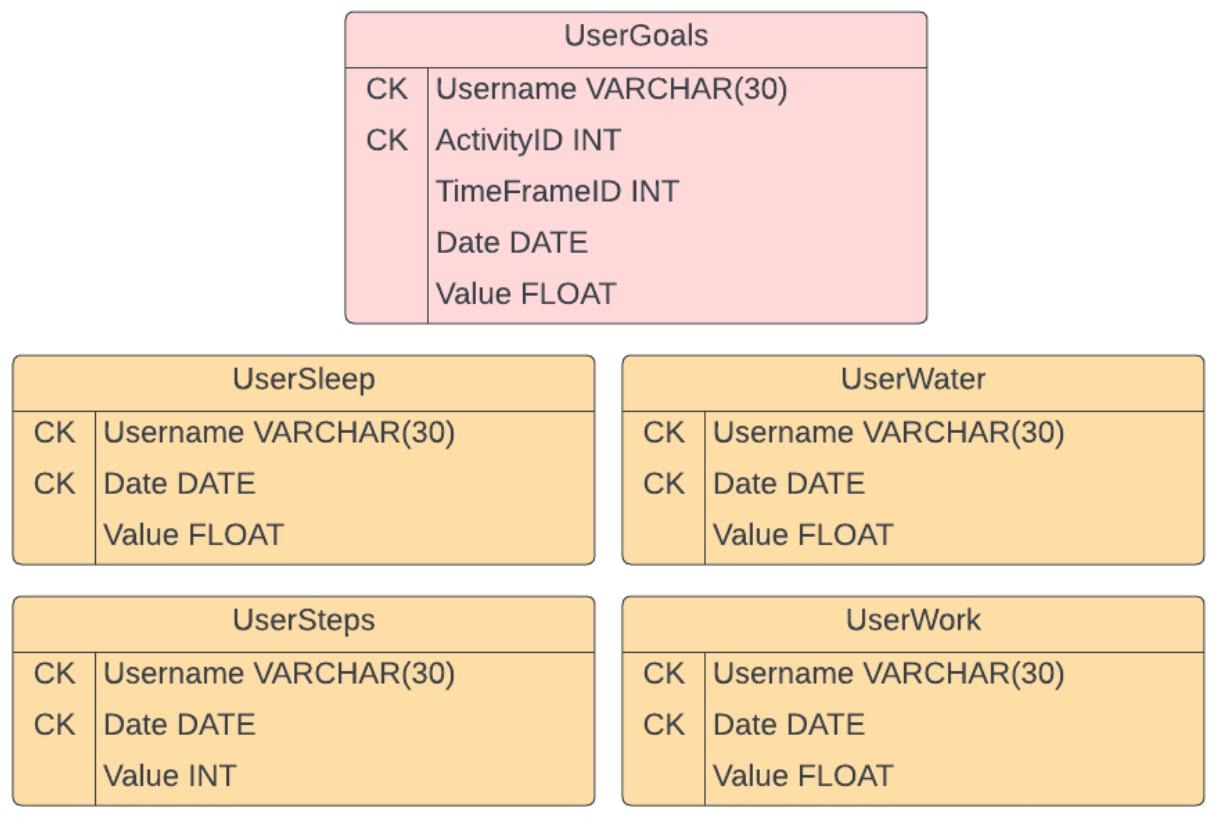
\includegraphics[width = 0.7\linewidth]{PI Systems Database}
  \caption{Database ERD Model}
  \label{fig:PI_ERD}
\end{figure}

Figure \ref{fig:PI_ERD} describes the following components:

\begin{itemize}

    \item \texttt{UserAchievements} Table: This table stores specific
        achievements of users, linked directly to the User table. Attributes
        like \texttt{Username}, \texttt{Date}, \texttt{ActivityID}, \texttt{TimeFrameID}, and \texttt{Value} allow for
        detailed recording and analysis of user accomplishments across
        different activities and timeframes. It enables the system to provide
        feedback and insights based on historical achievement data, supporting
        motivational features such as goal setting and progress tracking. This 
        table aimed to adhere specifically to SRQ 7.4, yet it also contributes to SRQ 7.1.\par

    \item \texttt{UserStep} Table: Dedicated to tracking the physical activity
        of steps taken, this table includes attributes such as \texttt{Username}, \texttt{Date},
        and \texttt{Value}. By recording daily step counts, the \texttt{UserStep} table feeds
        into the system’s health monitoring and fitness tracking capabilities,
        allowing users to set and monitor physical activity goals. As the data 
        can also be inserted though an API, this table aims to cover ARQ 2.\par

    \item \texttt{UserSleep} Table: Focusing on sleep habits, this table
        records the duration of sleep per day for each user with attributes
        \texttt{Username}, \texttt{Date}, and \texttt{Value}. It is vital for analysing sleep patterns
        and correlating them with other health metrics, which is essential for
        offering personalised health insights and improving user
        well-being.\par

    \item \texttt{UserWork} Table: This table tracks work and study sessions,
        an essential feature for our users. Attributes include
        \texttt{Username}, \texttt{Date}, and \texttt{Value}, facilitating the tracking of
        academic and work-related activities over time. This functionality
        supports users in managing their time and productivity more
        effectively.\par

    \item \texttt{UserWater} Table: Monitoring hydration, the \texttt{UserWater} table
        includes attributes such as \texttt{Username}, \texttt{Date}, and \texttt{Value}. Hydration
        tracking is crucial for overall health, and this table allows the
        system to remind users to stay hydrated and track their daily water
        intake.\par

    \item \texttt{UserGoals} Table: As a strategic component of our system, the
        UserGoals table holds data related to the personal objectives of users.
        With attributes like \texttt{Username}, \texttt{ActivityID}, \texttt{TimeFrameID}, \texttt{Date}, and
        \texttt{Value}, this table supports the setting and monitoring of personalised
        goals, enhancing the system's capability to drive user engagement and
        encourage behaviour modification. \texttt{UserGoals} covers SRQ 7.1, 7.2 and
        7.3.\par

\end{itemize}

\texttt{UserStep}, \texttt{UserSleep}, \texttt{UserWork} and \texttt{UserWater}
are all aimed to satisfy ARQ 5 and SRQ 5.1, 5.2 and 5.3.

\begin{figure}[!ht]
  \centering
  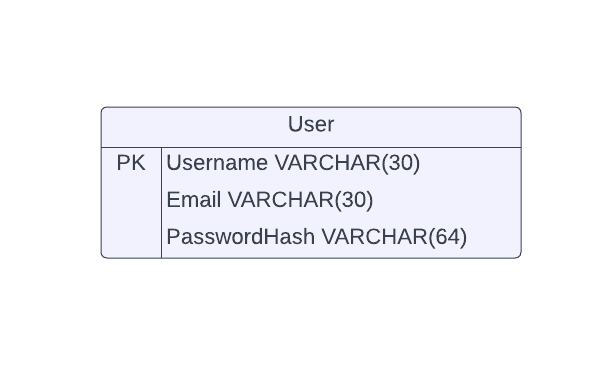
\includegraphics[width = 0.4\linewidth]{PI Systems Database-2}
  \caption{User Class in the Database Model}
  \label{fig:User_Table}
\end{figure}

Figure \ref{fig:User_Table} describes our \texttt{User} Table: used to be
central to our system, the User table captures essential personal identifiers and
account information for each user. Attributes include \texttt{Username}, \texttt{Email}, and
\texttt{PasswordHash}, which are fundamental for ensuring secure user authentication and
system access. This table acts as the primary entity with which other tables
associate, establishing a one-to-many relationship across various data-tracking
entities. Each instance of a user can associate with multiple records in
subordinate tables, reflecting the diverse activities and metrics tracked by the
system. Ultimately, the requirement for a multi-user system was omitted due to
limitations in the allocated time frame. However, the underlying database
architecture has been deliberately designed to facilitate the seamless
integration of multi-user capabilities, should they be developed in the future.
This table covers ARQ 1.

\subsection{UML Class Diagram}

\begin{figure}[!ht]
  \centering
  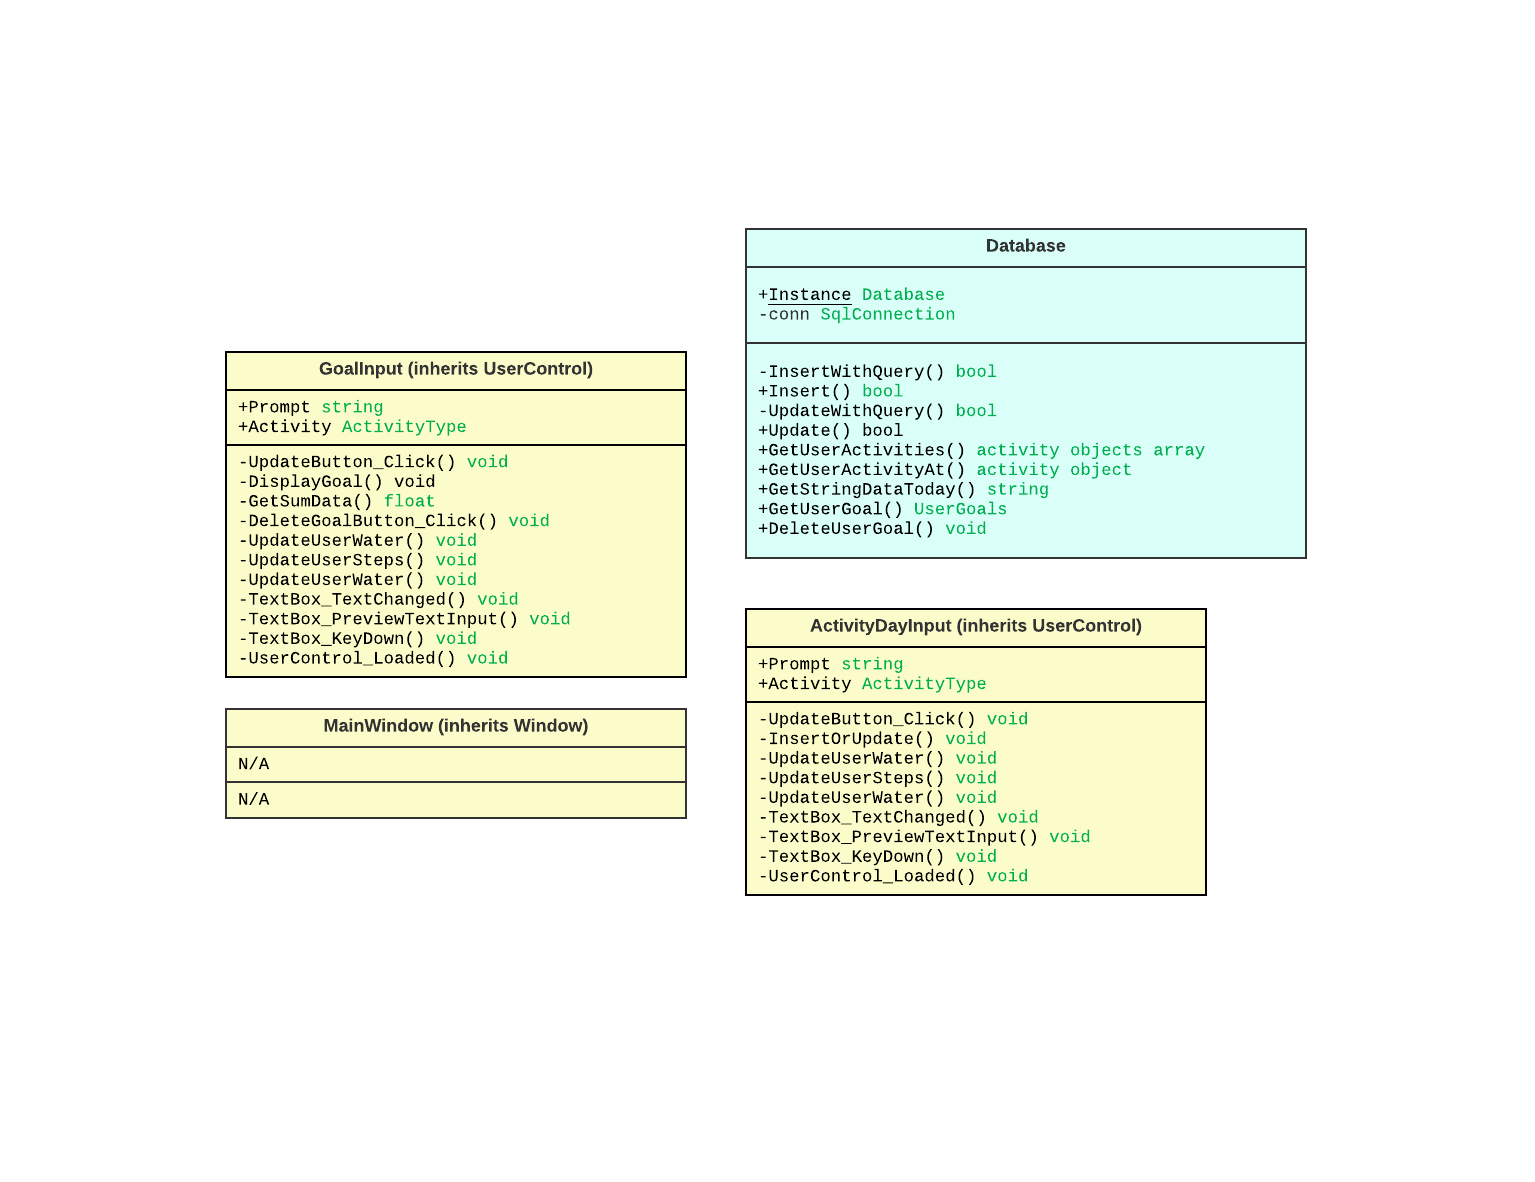
\includegraphics[width = 0.7\linewidth]{UML Class diagram}
  \caption{UML Class Diagram}
  \label{fig:Class}
\end{figure}

The class diagram of our PI system (Figure \ref{fig:Class}) delineates the
fundamental components and their relationships, underscoring the system's
design to efficiently manage and process user data. Central to this
architecture is the \texttt{Database} class, which acts as the primary conduit for all
data manipulation and retrieval activities within the system. This class is
critical for the robust handling of data and supports various functionalities
critical to user interaction and data integrity. We utilise the Dapper module 
in C\#, which facilitates the direct return or insertion of a list of 
C\# objects from an SQL query, rather than handling them as tuples. 
Accordingly, based on the ERD, all classes are designed to integrate seamlessly
with the Dapper package.\par

The \texttt{Database} class ensures a singleton pattern for database management,
creating a single, globally accessible instance throughout the application
lifecycle. It manages the database connectivity, facilitating secure and
persistent connections to the data store. Data manipulation methods such as
\texttt{InsertWithQuery()}, \texttt{Insert()}, \texttt{UpdateWithQuery()}, and \texttt{Update()} allow for
efficient data insertion and updating within the database. Retrieval methods
like \texttt{GetUserActivities()} and \texttt{GetUserActivityAt()} fetch activity data for users,
crucial for generating reports and insights. Utility methods including
\texttt{GetStringDataToday()}, \texttt{GetUserGoal()}, and \texttt{DeleteUserGoal()} provide additional
functionality for managing daily data strings and user goals, enhancing the
system’s responsiveness to user interactions. These methods were essential for
SRQ 6.1 and 6.2, as well as directly adhering to SRQ 5.1 and 5.2. \par

The \texttt{ActivityDayInput} and \texttt{GoalInput classes}, are specifically
designed for handling the input and update functionalities related to daily
user activities and goal management, respectively. The
\texttt{ActivityDayInput} Class includes a Prompt string for user guidance and
an Activity \texttt{ActivityType} to specify the type of activity data being
entered. It comprises various user interaction handlers such as
\texttt{UpdateButton\_Click()} and \texttt{InsertOrUpdate()} for data
submission, alongside \texttt{UpdateUserWater()} and \texttt{UpdateUserSteps()}
for updating specific activity metrics. Text handling methods like
\texttt{TextBox\_TextChanged()}, \texttt{TextBox\_KeyDown()} and
\texttt{TextBox\_PreviewTextInput()}. ensure data integrity and user input
validation.\par

The GoalInput Class mirrors the ActivityDayInput class in providing prompts and
activity type specifications tailored towards user goals. It features
goal-specific functionalities such as \texttt{DisplayGoal()} for visualising set goals,
\texttt{GetSumData()} for data aggregation, and \texttt{DeleteGoalButton\_Click()} for
goal modification. It inherits text handling and initialisation methods from
ActivityDayInput, ensuring a consistent and user-friendly interface. Whilst
ActivityDayInput stands mainly by SRQ 6.1 and 5.1, GoalInput follows SRQ 7.1, 7.2 and 7.3.\par

\subsection{UML Flow Diagram}

\begin{figure}[!ht]
  \centering
  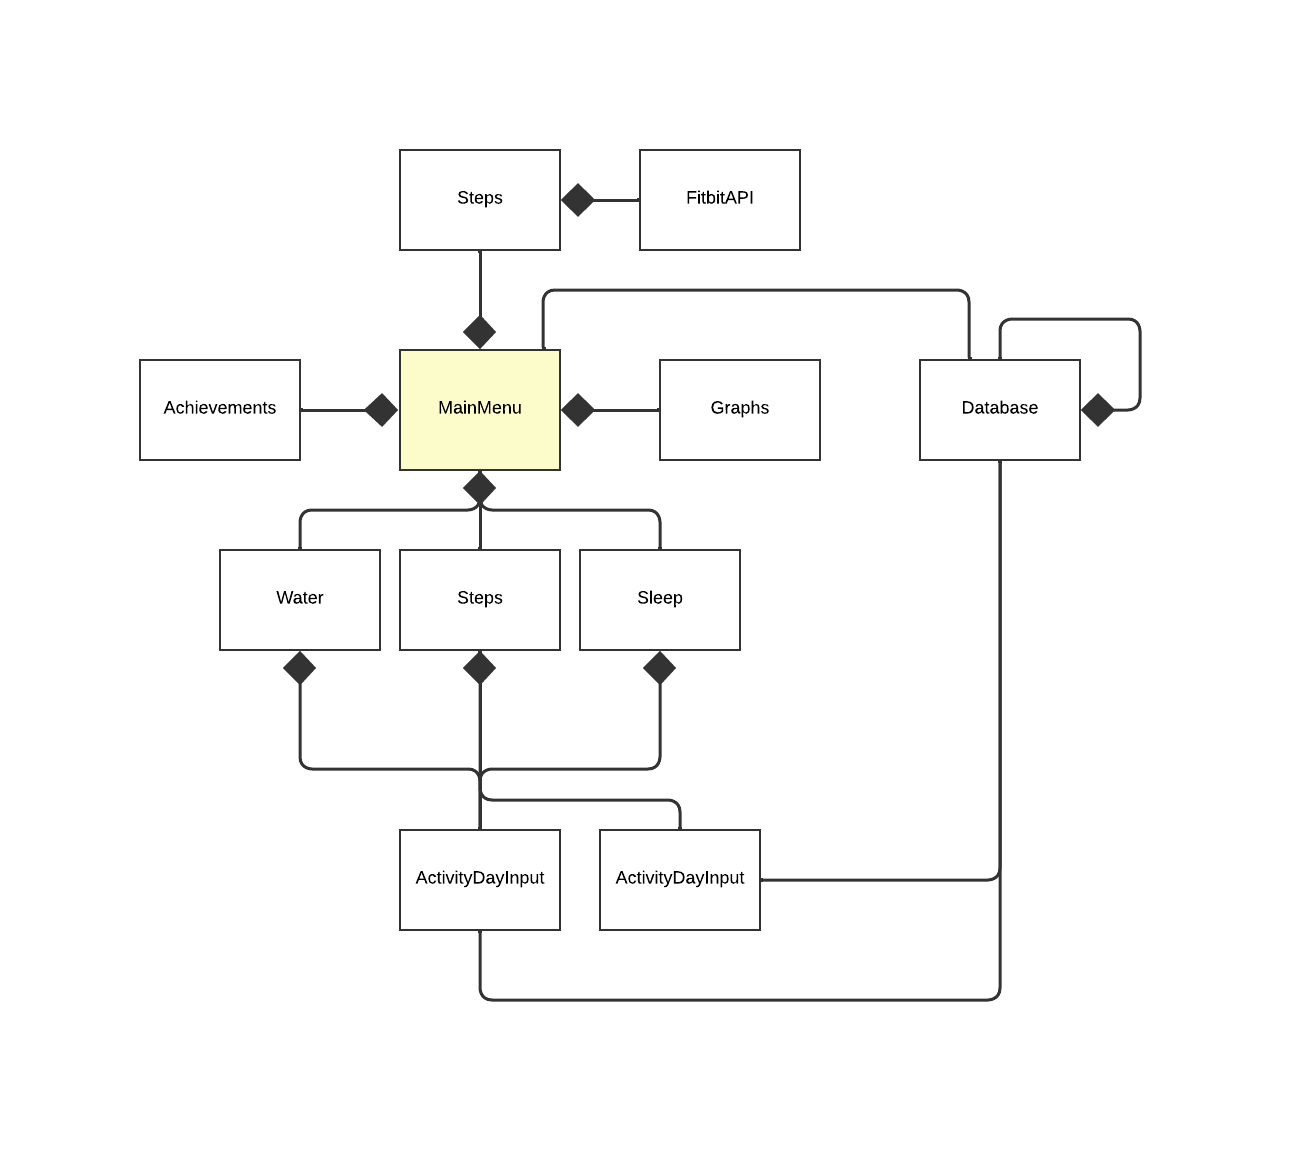
\includegraphics[width = 0.7\linewidth]{UML Flow diagram}
  \caption{UML Flow Diagram}
  \label{fig:flow}
\end{figure}

The flow diagram of our PI system (Figure \ref{fig:flow}) illustrates the
interactions between classes, essential for efficient functionality and user
experience. At the core is the MainMenu class, which integrates features like
tracking steps, achievements, water intake, and sleep via separate classes
(Step, Achievement, Water, Sleep). These classes manage specific activities and
are tightly integrated with \texttt{ActivityDayInput} and \texttt{GoalInput} controls for data
entry and goal management.\par

For example, when users input their daily water intake through the
\texttt{ActivityDayInput} tailored for water, this control processes and validates the
data, then interacts with the Water class and the Database to store this
information. Similarly, the \texttt{GoalInput} facilitates setting and updating goals,
interacting directly with the Database to ensure goals are current and
reflective of user activity.\par

The association between the \texttt{ActivityDayInput}, \texttt{GoalInput}, and the \texttt{Database}
ensures immediate data reflection in the system, supporting features like
activity comparison and trend analysis. The \texttt{Database} manages its instance,
maintaining data integrity and security, and acts as a centralised repository
for all user data. This structure ensures seamless data flow across the system,
fulfilling functional and non-functional requirements, and enhancing overall
user interaction. The association between these elements are the groundwork for all requirements SRQ 5, SRQ 6 and SRQ 7, as well as ARQ 4.\par

\subsection{User Interface}

This section outlines the design of the user interface (UI) for our PI system,
focusing on creating an intuitive and engaging user experience. We aim to bridge
the gap between the system's technical capabilities and the user's needs through
a well-thought-out interface. The UI design is crafted to facilitate easy
navigation and interaction, ensuring that users can efficiently manage and track
their personal data. Here, we discuss the guiding principles of our UI design and
how they enhance usability and user engagement.\par

\begin{figure}[!ht]
  \centering
  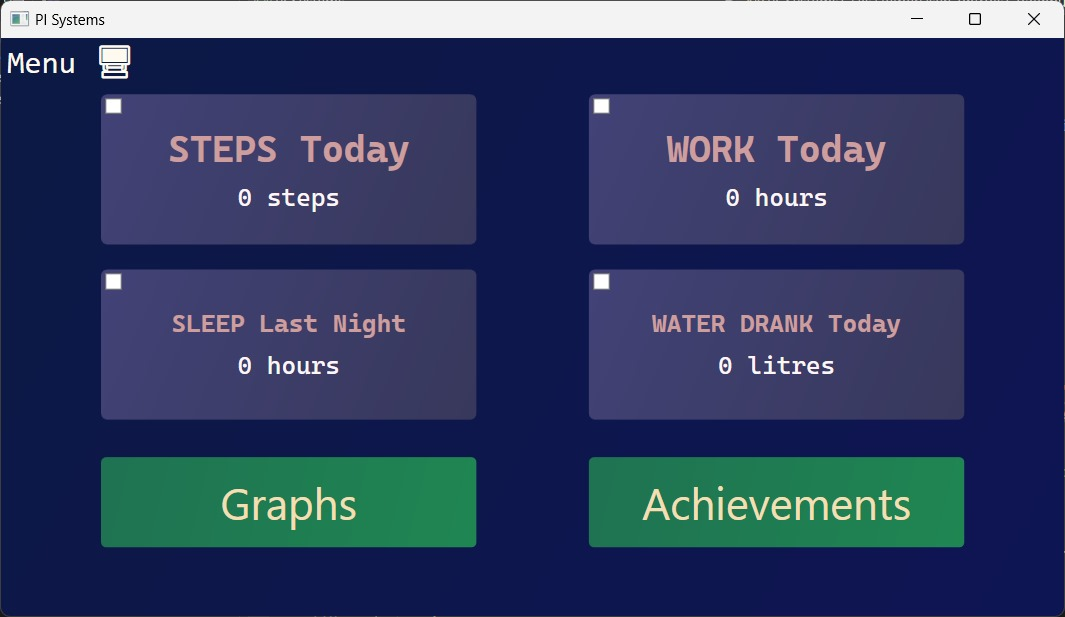
\includegraphics[width = 0.5\linewidth]{Main Menu}
  \caption{Main Menu of the Application}
  \label{fig:Menu}
\end{figure}

Figure \ref{fig:Menu} illustrates the main menu of our application. Positioned in the top left
corner of the screen, the label \texttt{"Menu"} accompanied by a small computer icon indicates
to the user that they are currently viewing the main menu. The background of the 
entire menu is a dark blue, a colour choice designed to minimise eye strain during 
prolonged use of the app.\par

The main menu features four prominent buttons, each corresponding to the core 
functionalities of the Personal Informatics system: steps, work, sleep, and water.
Additionally, two smaller green buttons provide access to sub-functionalities, 
specifically graphs and achievements. Each of the four larger buttons displays 
the type of statistic it relates to, with today's data (or the previous night's
for sleep hours) shown in smaller font size directly below. The design adheres to SRQ 5.2 and 6.1.\par

A unique aspect of the design is a small white checkbox located in the top left
corner of each button. These boxes can be marked by user when they want to see
the related data in graph, and therefore allows for SRQ 6.2 to function smoothly.
Moreover, several boxes can be ticked at once, allowing users to see the relativity of different type of stats in one graph.\par

\begin{figure}[!ht]
  \centering
  \begin{subfigure}{0.4\linewidth}
    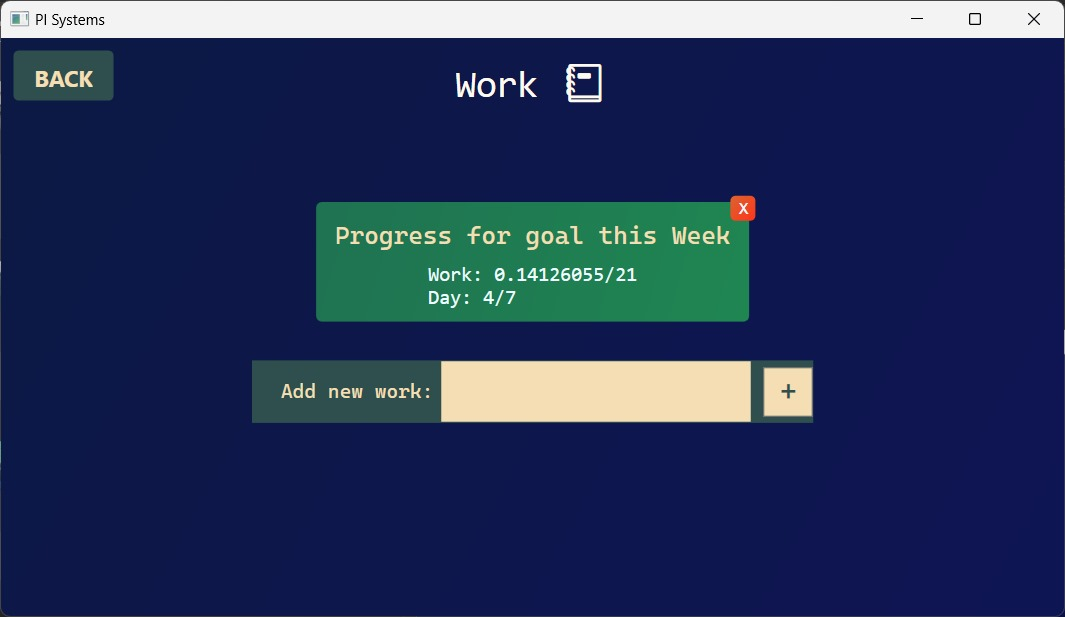
\includegraphics[width = \linewidth]{Work Screen}
    \caption{Work Section Interface}
    \label{fig:Work}
  \end{subfigure}%
  \vspace{10pt}
  \hfill
  \begin{subfigure}{0.4\linewidth}
    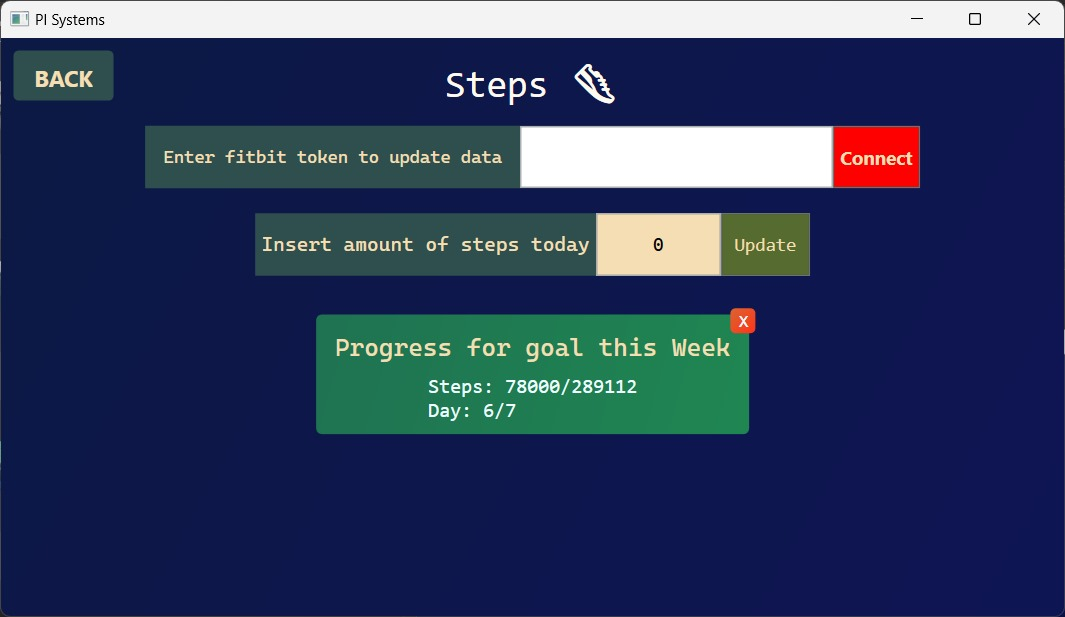
\includegraphics[width = \linewidth]{Steps Screen}
    \caption{Steps Section Interface}
    \label{fig:Steps}
  \end{subfigure}

  \begin{subfigure}{0.4\linewidth}
    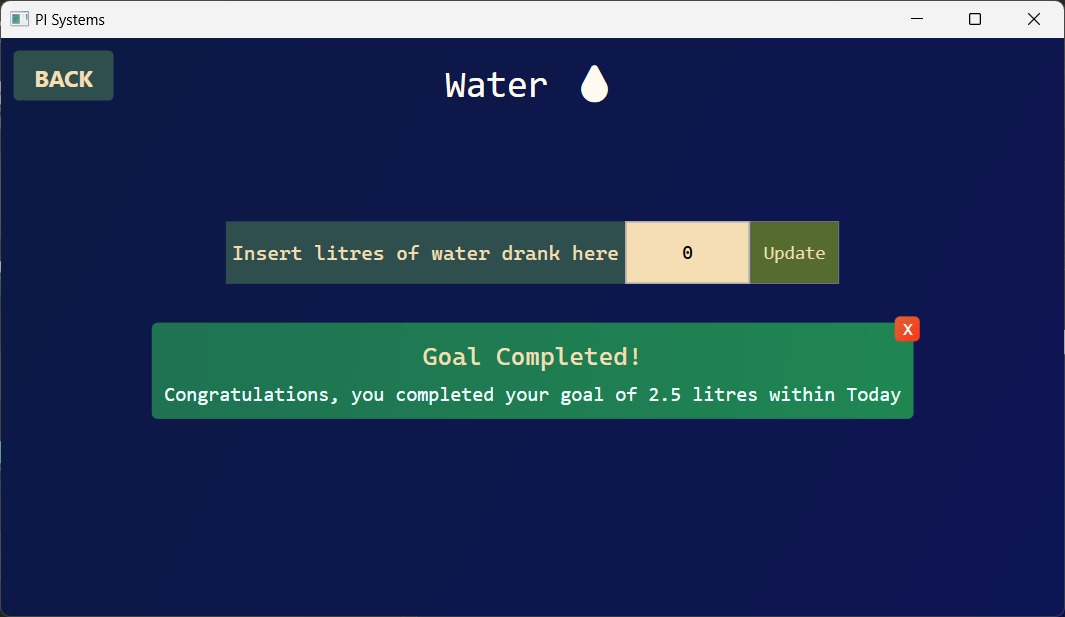
\includegraphics[width = \linewidth]{Water Screen}
    \caption{Water Section Interface}
    \label{fig:Water}
  \end{subfigure}%
  \hfill
  \begin{subfigure}{0.4\linewidth}
    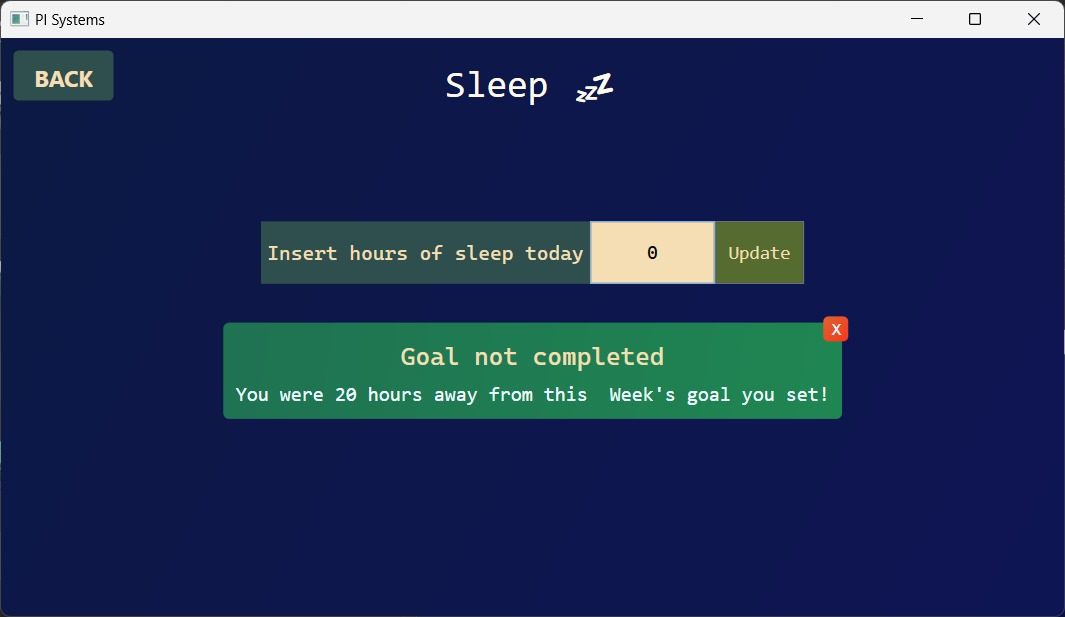
\includegraphics[width = \linewidth]{Sleep Screen}
    \caption{Sleep Section Interface}
    \label{fig:Sleep}
  \end{subfigure}

  \caption{Main Functionalities Interface}
  \label{fig:Main}
\end{figure}



Figure \ref{fig:Main} displays the four main functionality screen, which is designed
to be simpler and more focused compared to the main menu. In the top left corner, a 
dark green \texttt{"BACK"} button allows users to easily return to the main menu.\par 

We can clearly see from figure \ref{fig:Work} that the heading \texttt{"WORK"} is
prominently displayed at the top of the screen, accompanied by a book icon to
visually represent the category. Centred on the screen is a large green box that
tracks and displays the user's progress on their weekly achievement goals. Under
the heading \texttt{"Progress for goal this Week"} of the box, the interface
shows the amount of work completed and the specific day of the week the goal was
set. This box can be closed using the small red \texttt{"x"} button located at
its top right corner, providing a way to dismiss the details if desired. Directly
below this display, there is an input bar where users can \texttt{"Add new work"}
they have completed that day. Adjacent to this bar, a plus button is the way to
confirm the work users inserted and start to time it, allowing users to easily
update their daily work achievements. This was designed in this format for ARQ 5.\par

\begin{figure}[!ht]
  \centering
  \begin{subfigure}{0.4\linewidth}
    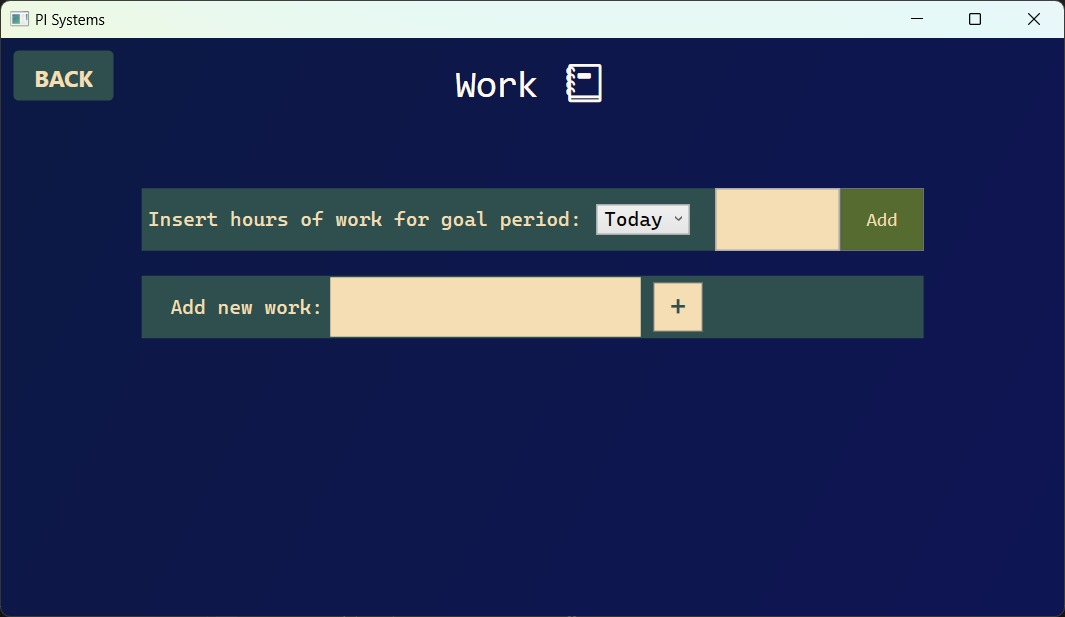
\includegraphics[width=\linewidth]{Add Work}
    \caption{Add Work bar}
    \label{fig:Add_Work}
  \end{subfigure}
  \hfill
  \begin{subfigure}{0.4\linewidth}
    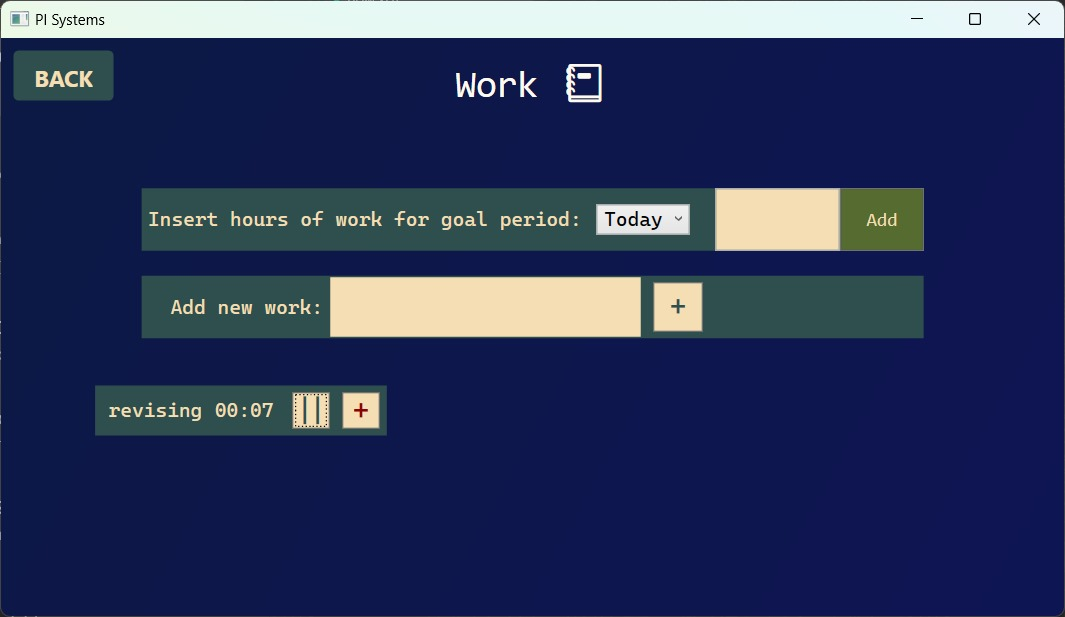
\includegraphics[width=\linewidth]{Add Work 2}
    \caption{Add work successfully}
    \label{fig:Add_Work_2}
  \end{subfigure}
  \caption{Add Work Interface}
  \label{fig:Work_Interface}
\end{figure}

Figure \ref{fig:Work_Interface} illustrates how the functionality Work works. When users dismiss
the progress box, the will see a new input bar, which they can use to add the amount of time that
they work for the time period they chose in the bar (figure \ref{fig:Add_Work}). Another way here
is to insert the type of work users want to do in the \texttt{"Add new work"} bar and then press 
the plus button. The work will appear and the time start running, users can pause it whenever they
like. After finishing the work, users can press the red plus button to add the time they have been
working for to the progress. They can easily check it in the main menu screen.\par

Figure \ref{fig:Steps} presents the steps interface, which maintains a consistent design
with the work screen but introduces several specific modifications. The heading \texttt{"Step"} is
displayed at the top of the screen, distinguished by a shoe icon next to it, replacing the
book symbol used in the work interface. A notable difference in layout is the placement of
the progress box, which is positioned below the input bars rather than above. This adjustment
allows for immediate and easy data entry upon accessing the screen, complying with ARQ 5.\par

\begin{figure}[!ht]
  \centering
  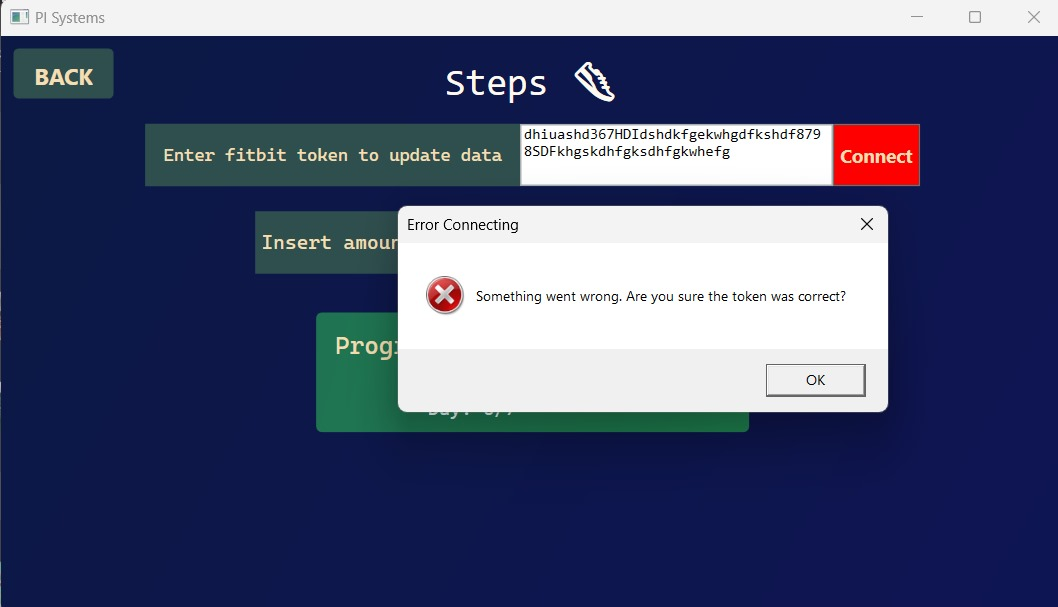
\includegraphics[width = 0.5\linewidth]{Error}
  \caption{Error inserting wrong API Token format}
  \label{fig:Error}
\end{figure}

Additionally, a new input bar for inserting an API token has been added to facilitate the integration of step data from
external devices or services and fulfilling ARQ 2. Directly next to the API token input bar are \texttt{"Connect"} and 
\texttt{"Update"} buttons. The \texttt{"Connect"} button is used for verifying the API token, while the \texttt{"Update"}
button adjacent to the Step input bar enables users to refresh and submit their step count 
data. Any incorrect format in the input will trigger an error message, as illustrated in 
figure \ref{fig:Error}, ensuring users are aware of input specifications and can correct their entries accordingly.\par

Figures \ref{fig:Water} and \ref{fig:Sleep} illustrate the design of the Water and Sleep screens,
respectively, which are consistent in layout with the other main functionalities of the app. 
Both screens feature a \texttt{"BACK"} button in the top left corner for easy navigation. The Water 
screen is identified by a heading labeled \texttt{"Water"} accompanied by a water drop icon, and the
Sleep screen is marked by a heading labeled \texttt{"Sleep"} adorned with a \texttt{"zzz"} icon. Each screen 
includes an input bar for users to enter their respective data values easily.\par

In Figure \ref{fig:Water}, showcasing the Water functionality, the progress box is displayed
upon achieving a set goal. It prominently features the message \texttt{"Goal Completed!"} in bold 
golden text, accompanied by a congratulatory message that also specifies the goal achieved.
This positive reinforcement is designed to motivate users and acknowledge their accomplishments, as SRQ 7.4 demands.\par

Conversely, Figure \ref{fig:Sleep} details the Sleep functionality when a goal is not met.
The progress box in this scenario displays a bold, golden headline \texttt{"Goal Not Completed"} at
the top. Below this heading, the screen informs users of the shortfall, specifying the 
amount needed to achieve the goal. In the depicted example, it indicates that the user 
was 20 hours short of reaching the weekly sleep goal. This feedback is intended to 
encourage users to adjust their habits to meet their sleep targets in the future.\par

\begin{figure}[!ht]
  \centering
  \begin{subfigure}{0.4\linewidth}
    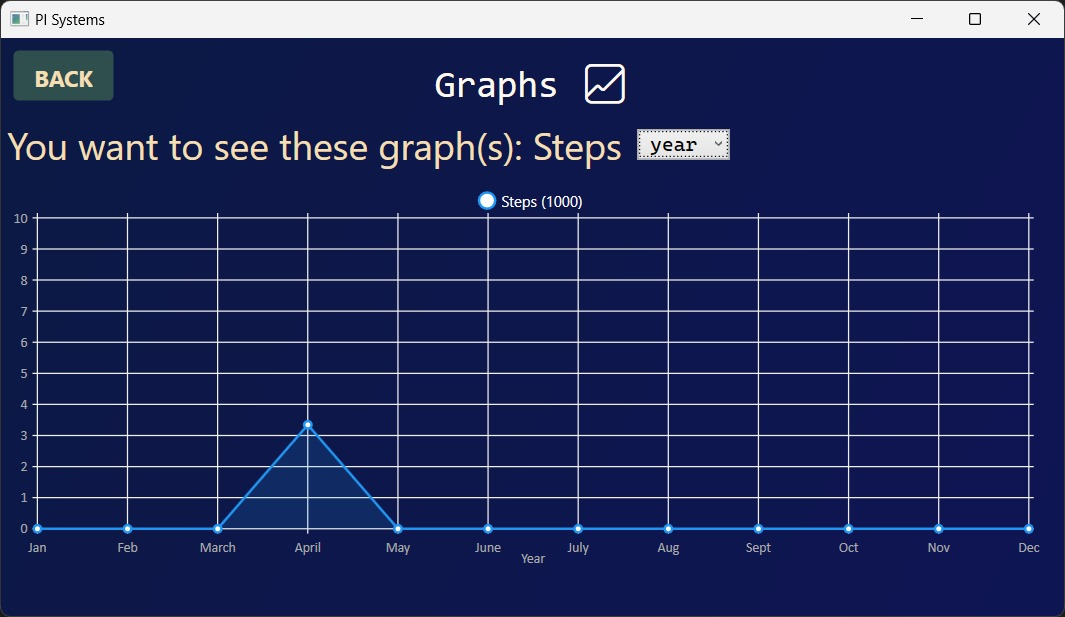
\includegraphics[width=\linewidth]{Graphs Screen}
    \caption{Graphs Section Interface}
    \label{fig:Graphs}
  \end{subfigure}
  \hfill
  \begin{subfigure}{0.4\linewidth}
    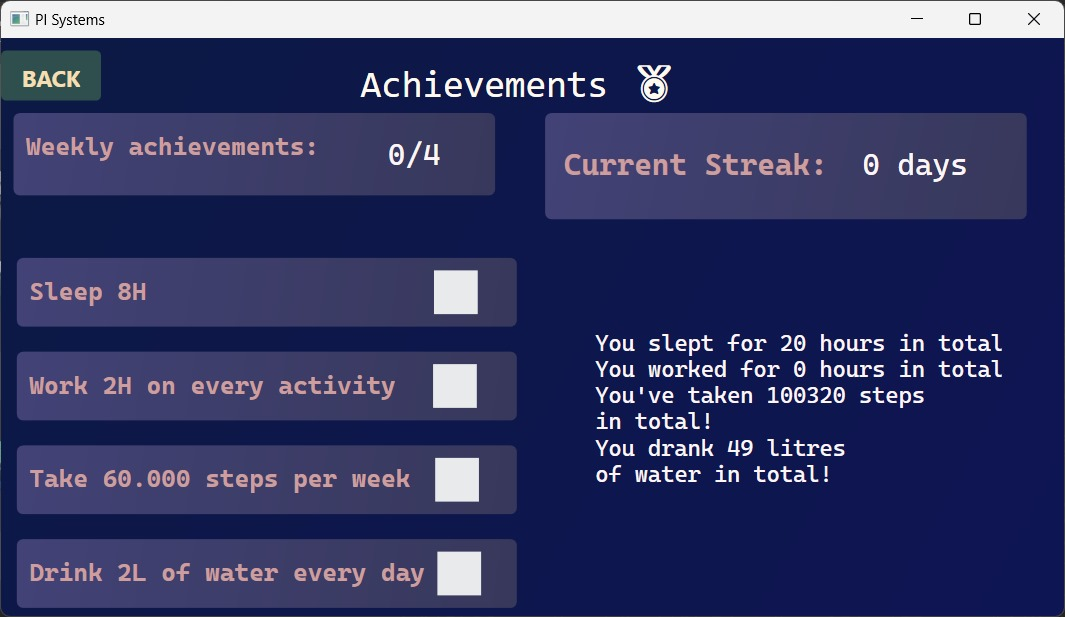
\includegraphics[width=\linewidth]{Achievements Screen}
    \caption{Achievements Section Interface}
    \label{fig:Achievements}
  \end{subfigure}
  \caption{Two other functionalities}
  \label{fig:subfunc}
\end{figure}

Figure \ref{fig:Graphs} showcases the Graph interface of the application, which is
designed to provide a visual representation of user data over time. The screen 
includes a \texttt{"BACK"} button located at the top left corner, allowing users to easily
navigate back to the main menu. The heading \texttt{"Graphs"}, marked with a small graph icon,
indicates the functionality of the interface.\par

The main feature of this interface is a large line graph, titled at the top to specify
the type of data being displayed. Users have the flexibility to select the timeline 
for the graph, ranging from a day to a year, with the current example set to display
data over a year. The timeline is plotted on the horizontal axis, while the specific
metrics related to the user’s activities are displayed along the vertical axis. The 
graph utilises a light blue line on a gridded white background, enhancing readability
and making it easier for users to interpret their data trends. The graph is also capable of showing multiple line at once with different colour. This feature makes it easier for users to compare among different types of statistic (figure \ref{fig:2_graphs}). Through this interface, SRQ 6.1 and 6.2 are followed.\par

\begin{figure}[h!]
  \centering
  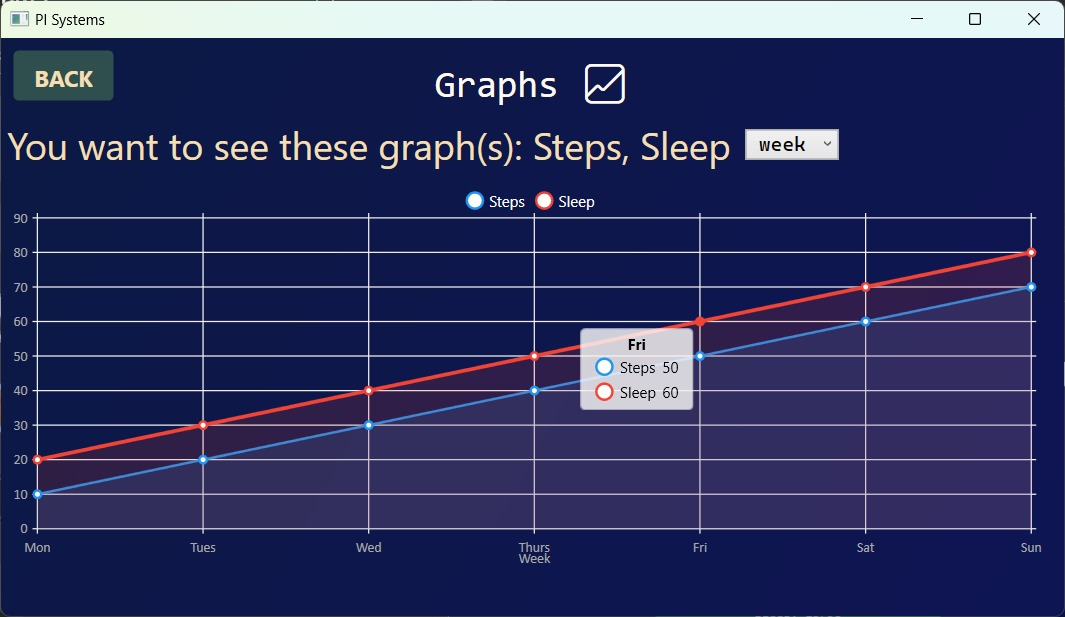
\includegraphics[width = 0.5\linewidth]{2 line graph}
  \caption{More than one line graph can be shown at a time}
  \label{fig:2_graphs}
\end{figure}

Figure \ref{fig:Achievements} presents the Achievements interface, which aims to motivate
and inform users about their progress in meeting set goals. Similar to other interfaces,
it includes a \texttt{"BACK"} button at the top left for returning to the main menu and is labeled
with the heading \texttt{"Achievements"}, accompanied by a medal icon to symbolise success and recognition.\par

The interface is divided into two main sections. On the left, a box at the top displays
the number of achievements completed within the week, indicated as \texttt{"0/4"} in this example,
suggesting no goals have been met yet. Below this summary, four boxes represent the 
achievements tied to the four main functionalities of the system (steps, work, sleep, and
water). Each box includes a white checkbox that is ticked off when the corresponding daily
goal is achieved.\par

On the right half of the screen, a white text box provides a summary of the total activities
completed for each functionality during the week, assisting users in tracking their weekly
progress. Additionally, a streak counter is placed above the activity summaries, encouraging
users to consistently meet their daily goals and build long-term habits.\par

Together, these interfaces support the app’s objective to engage users actively in tracking
their progress and achieving their health and productivity goals, perfectly complying with SRQ 7.1 and allowing users to compare data with others, complying with ARQ 1.\par


\section{Software Testing and Verification} \label{sec:testing}

During the initial planning of this project, the approach to testing was
discussed and a Test Plan was created,  Figure \ref{fig:TestDesign} . It was
agreed that each time a developer completed a feature from the product backlog
they would thoroughly white-box test it themselves using a variety of
specifically chosen test cases and take screenshots to record the results. If
all tests produced the desired results, the developer would consider the
feature complete. If any tests were unsuccessful, however, they would debug and
fix the problem before applying all tests again.  If the error was found in
anothers developers code,  the error and the test results were provided to the
person responisble and they would colaborate on the debugging.  In this way,
the component's functionality given both valid and invalid inputs would be
ensured. By testing each element before combining it with other elements of the
system, the testing process as a whole would comprise a bottom-up integration
testing approach. On the completion of a part of the product backlog, the
developer would send the screenshots produced in testing to the product owner.
The product owner would then analyse the screenshots to ensure that the
evidenced functionality aligned with the requirements of the product backlog.
The product owner would also use the screenshots to provide feedback to the
developers and to inform future decisions and alterations to the product
backlog.\par

\subsection{Examples}

The programmers in our group were very good at ensuring that their code
initially contained no bugs so testing revealed very few errors. Below,
however, are some examples of bugs that were found which demonstrate how
effective the testing approach was in ensuring the adherence of our system to
the specifications and the smooth operation of the software.\par

\subsubsection{Achievement Consistency}
When testing the achievements section of the product, the following test 
cases were included in the process:\par
\begin{center}
    \begin{tabular}{|p{5cm}|p{5cm}|p{5cm}|}
        \hline
        \textbf{Description} & \textbf{Test} & \textbf{Expected Result}\\
        \hline
        Achievement page highlights completed achievements & Input data which 
        completes an achievement & Achievement page highlights completion and 
        shows correct progress \\
        \hline
        Achievement page does not highlight previously completed achievements 
        which are no longer complete & Input data which completes an achievement 
        then edit data so that achievement is not completed & Achievement page 
        reverts highlighting and progress label\\
        \hline
    \end{tabular}
\end{center}
The first test of the two was passed successfully. However, while the progress 
label did revert to a lower value upon alteration of the data, the achievement 
remained highlighted, as shown in figure \ref{fig:ManualTest1}(see Apendix).\par

 %Image removed 

The developer in charge of this section was quickly able to find the source of 
this issue and fix it.\par

\subsubsection{Incomplete Input}
Another issue that was found during testing was in the manual data input. To avoid 
invalid entries, the input box only allowed numbers and decimal points to be entered, 
however, the following test case caused an unexpected error.\par
\begin{center}
    \begin{tabular}{|p{5cm}|p{5cm}|p{5cm}|}
        \hline
        \textbf{Description} & \textbf{Test} & \textbf{Expected Result}\\
        \hline
        Incomplete inputs are handled gracefully 
        & Input a decimal point 
        & Input is treated as a zero\\
        \hline
    \end{tabular}
\end{center}

%Image removed

When a decimal point was entered,  as in figure \ref{fig:ManualTest2}(see Apendix), the program froze and then crashed. 
To avoid this, the developer changed the code handling the inputs and 
the problem was solved.\par

\subsubsection{Goal Expiry}
A third example of an error caught by our testing was an issue with the 
time period of goals. During testing, the following test case failed:\par
\begin{center}
    \begin{tabular}{|p{5cm}|p{5cm}|p{5cm}|}
        \hline
        \textbf{Description} & \textbf{Test} & \textbf{Expected Result}\\
        \hline
        Goals expire once end time has been reached 
        & Allow a goal to end uncompleted 
        & Goal shows failure and ends\\
        \hline
    \end{tabular}
\end{center}

% Image removed

As shown in the figure \ref{fig:ManualTest3}(see Apendix), once the goal time had passed, the counter 
simply continued to run. This relatively major issue was quickly resolved 
and the feature now functions correctly.\par

\section{Reflection and Conclusion}

With our PI system now complete and the specified requirements met, we can 
reflect on the merits and failures of the system and our approach to it. To do 
this we will critically analyse the way our system was designed and specified, 
as well as the approach we followed during development. By doing this we will 
be able to conclude as to the success of this project as a whole, consider 
future alterations to our system and analyse ways in which our approach could 
be improved. Learning from this, we will be able to develop systems more 
successfully in the future. Unfortunately, due to the deadline for the 
completion of our  project, we will not be able to try using our system for a 
significant period of time in order to properly gauge how well it works from 
a user's perspective but, we can still evaluate it from a critical viewpoint 
and make educated speculations about its effectiveness.\par

\subsection{System Development}
The creation the specification for our system began with research to establish 
the interests of our target demographic. The biggest parts of this research 
were an online form distributed to our peers and some interviews. The results 
of these were very helpful and were the driving force behind our choice of 
tracking metrics. However, while this approach was sound and successful in 
gathering information, only around twenty individuals filled in the form and 
we only managed to interview two individuals. This is a large enough number of 
people that we feel comfortable with using the results as a guide, especially 
given the clear majority in the opinions of the form respondents. However, in 
future, ensuring a larger sample size would improve the reliability of our 
results and, at the very least, make us more certain in our decisions.\par

Our choice of tracking metrics was informed both by data gathering and by 
research into other PI systems. This meant that our final list of four metrics 
reflected the desires of our peers, as well as our informed opinions on the 
most beneficial choices. On reflection, these four metrics still seem to 
provide an excellent and balanced summary of an individual's physical and 
mental health in a way that appears likely to provide useful insights and 
achievable targets. We are therefore confident that our choice of metrics is 
sound. However, due to the variety of research responses, especially from the 
interviewees, it was not possible to take the views of every individual into 
account; there were a few features suggested during the interviews which were 
not added to the specification, either due to the need to limit the scope of 
the system or because they didn't align with the conclusions of other 
respondents or with our research. In future, looking back on this research or 
through conducting more thorough research, we could implement extra features 
over a longer period if a consensus was reached among requests.\par

One key requirement we specified for our system, which is a very important 
feature of any PI system, was the ability to log data. This specification was 
clearly met, with the user able to log their progress in all four metrics. The 
manual data entry process is also very simple and intuitive, with very little 
room for confusion. By implementing it in this way we have made the data entry 
aspect of our PI system as effortless as possible, thereby making the use of 
our system more pleasant for the user. The system also has the ability to use 
the Fitbit API to gather data, as specified in the requirements. While this 
does work well and fulfils the requirements, Fitbit refresh API tokens on a 
regular basis. This means that users are regularly required to re-enter their 
Fitbit API token for our system to gather their data, reducing the benefits of 
the automated tracking. In future, it would be beneficial to look into 
avoiding this problem so that the effort required on the part of the user is 
minimised. Avoiding this is presumably possible as the Fitbit mobile app is 
reportedly built using this API and does not require repeated token entry from 
users.\par

Another important PI feature which our specification detailed was the 
intuitive display of user data and progress. This requirement was successfully 
met through the use of a software library specialising in graphs. Using this, 
aesthetic, interactive and detailed graphs for chosen metrics were produced, 
giving users insight into health variations in their lifestyle. A possible 
area for improvement in this section would be the highlighting of particularly 
healthy periods of time to motivate the user, as this has been shown to promote 
positive reflection (Loerakker et al., 2023). However, the functionality of 
this feature certainly meets the requirements we set out.\par

The principal other feature our specification required was the inclusion of 
goals and achievements. This was also successfully implemented and provides 
an effective way to track progress towards goals and to provide motivation, 
making it a worthwhile part of the specification and the system. In future, 
however, a possible improvement would be the ability to see other users' 
achievements within the application. Of course, successes can be compared by 
the sharing of screenshots or in-person demonstration but a built-in system 
would make this easier and could help spread word of the system to more 
students who might find it useful. Additionally, the ability to have multiple 
goals per activity could be beneficial for some users. For example those who 
would like to have a short-term goal and a longer term goal.\par

The database our system uses is designed to integrate intuitively with the 
structure of our software and is quick and easy to understand and access. The 
addition of future metrics to our system would not be difficult to implement, 
simply requiring an associated table. However, while our database is intuitive, 
it could be normalised further by adding a bridging table with 
activity IDs. The benefit of this change would be increased efficiency and 
ease of further development. Adding new metrics would likely only require an 
extra record in the Activities table. However, there would also be downsides 
to this approach; understanding the layout of the database would be less 
simple, relying on keeping track of foreign keys and more complicated database 
queries. Our class design closely resembles that of our database and is 
therefore similarly intuitive. If we were to alter the database design, 
careful alterations to the interface between the database and the code could 
maintain the clarity of data storage from a programming perspective by 
minimising changes in the class design.\par

As per our specification, the PI system is a locally-run PC application. This 
is beneficial to users when it comes to the viewing of the graphical statistics 
provided by the program as the majority of computers running the program will 
likely have a larger screen than a tablet or smartphone. However, it also 
requires that users log data using a large device. This could become quite 
burdensome, especially when away from home, because of the requirement for a 
laptop running the system. Given the widespread use of smartphones which are 
often carried almost everywhere, a future improvement to our system would be 
to allow the tracking of data on mobile devices, making the process much more 
portable and accessible.\par

Our approach to the test-driven development of our system worked well in 
practice, with developers finding most of the bugs in their own code during 
testing and the finished product working effectively with no known issues. By 
using white-box testing the developers were able to apply tests based on their 
in-depth knowledge of the processes involved, thereby anticipating problems 
others would not. However, on one occasion, a bug went unnoticed by the initial 
testing and was only picked up by the product owner. This implies that, in 
future, a combination of white-box and black-box testing might prove to be more 
robust due to the diverse perspectives provided by group work.\par  

\subsection{Software Process}
To develop this product we followed the Scrum framework and the Agile 
methodology of software development with the aim of allowing us to structure 
and manage the creation of the system in an effective and methodical way. We 
managed to complete five week-long sprints during the development process with 
the sprint backlog successfully cleared during the majority of the sprints and 
almost cleared during the rest.  This process definitely helped us to keep 
track of our progress in comparison with the specification and kept us to an 
efficient schedule which kept development moving at a sensible pace. It also 
allowed the system requirements to evolve during development, leading to a 
better final product overall.\par

One way in which we could have improved our adherence to the Scrum framework 
would have been the inclusion of more frequent Scrum meetings. During our 
sprints, frequent Scrum meetings were held to discuss progress but they did 
not always occur on a daily basis. Holding daily scrum meetings would have 
been impossible given our busy and clashing schedules, especially during 
the Easter Break when developers had significant plans outside of work. 
However, more Scrum meetings could have been held on occasion and may have 
improved communication and understanding within the group.\par

A notable way the Agile methodology allowed us to evolve our requirements 
was in the design of the system's database. In a sprint planning session 
part way through the development process, it was realised that our database 
could be made more efficient by adjusting the design. The product 
backlog was updated to include this new design and the change was implemented 
as part of the sprint that followed, making the database more efficient. In 
this way, the Agile methodology helped us avoid future problems and work by 
allowing flexibility during the development process\par

A part of the process that worked particularly efficiently in our group was 
the sprint planning weekly meetings. By having a member of the team run the 
meetings, and through open communication, we managed to always ensure that 
every member of the team had something to do and could work on them 
effectively during the sprint so that the group as a whole produced 
meaningful results during the sprint and finished the project before 
the deadline.\par

\subsection{Conclusion}
In conclusion, through carefully considered design and adherence to Agile 
methods, we managed to successfully produce a working PI system in an 
organised way. We believe that this system is intuitive, informative and 
robust. Furthermore, our approach to testing and development was 
effective, however testing may have been improved by incorporating a more collaborative system. Therefore, the development of this system has primarily been a 
success. However, there are areas in which the system itself could be 
improved in future to increase ease of use, which given a longer development time could have been addressed accordingly.\par

\newpage
\section{References}

\renewcommand{\refname}{} 
\vspace{-20pt}
\begin{thebibliography}{99}
    \bibitem{jones-2018}Jones, S. L. and Kelly, R., 2018. 
    Dealing With Information Overload in Multifaceted Personal Informatics Systems. 
    \textit{Human–computer interaction}, 33(1), pp. 1–48. \url{https://doi.org/10.1080/07370024.2017.1302334}

    \bibitem{kersten-van-Dijk-2017}Kersten-van Dijk, E. T., Westerink, J. H. D. M., Beute, F. and 
    IJsselsteijn, W. A., 2017. 
    Personal Informatics, Self-Insight, and Behavior Change: A Critical Review of Current Literature. 
    \textit{Human–computer interaction}, 32(5–6), pp. 268–296.

    \bibitem{potapov-2021}Potapov, K., Vasalou, A., Lee, V. and Marshall, P., 2021. 
    What do Teens Make of Personal Informatics? 
    Young People's Responses to Self-Tracking Practices for Self-Determined Motives. 
    \textit{Proceedings of the 2021 CHI Conference on Human Factors in Computing Systems}, 
    8-13 May 2021, New York. Association for Computing Machinery, pp. 1–10.

    \bibitem{loerakker-2023}Loerakker, M.B., Niess, J., Bentvelzen, M. and Woźniak, P.W., 2023. 
    Designing Data Visualisations for Self-Compassion in Personal Informatics. 
    \textit{Proceedings of the ACM on interactive, mobile, wearable and ubiquitous technologies}, 7(4), pp. 1–22.

    \bibitem{madore-2019}Madore, K. P. and Wagner, A. D., 2019. Multicosts of Multitasking. 
    \textit{Cerebrum:the dana forum on brain science}[Online], 4(19). Available from:
    \url{https://www.ncbi.nlm.nih.gov/pmc/articles/PMC7075496/#sec-a.c.ftitle} 
    [Accessed 5 April 2024]

    \bibitem{nhs-2023}National Health Service, 2023. \textit{Water, drinks and hydration} [Online] 
    Available from: 
    \url{https://www.nhs.uk/live-well/eat-well/food-guidelines-and-food-labels/water-drinks-nutrition} 
    [Accessed 5 April 2024]
    
    \bibitem{rapp-2016}Rapp, A. and Cena, F., 2016. Personal informatics for everyday life: 
    How users without prior self-tracking experience engage with personal data. 
    \textit{International journal of human-computer studies}, 94, pp. 1-17

    \bibitem{tudor-locke-2011}Tudor-Locke, C., Craig, C. L., Brown, W. J., Clemes, S. A., De Cocker, K., 
    Giles-Corti, B., Hatano, Y., Inoue, S., Matsudo, S. M., Mutrie, N., Oppert, J. M., Rowe, D. A., 
    Schmidt, M. D., Schofield, G. M., Spence, J. C., Teixeira, P. J., Tully, M. A. and Blair, S. N., 2011. 
    How many steps/day are enough? For adults. 
    \textit{The international journal of behavioral nutrition and physical activity} 
    [Online], 8(79). Available from: \url{https://doi.org/10.1186/1479-5868-8-79}

    \bibitem{watson-2015}Watson, N. F., Badr, M. S., Belenky, G., Bliwise, D. L., Buxton, O. M., Buysse, D., 
    Dinges, D. F., Gangwisch, J., Grandner, M. A., Kushida, C., Malhotra, R. K., Martin, J. L., Patel, S. R., 
    Quan, S. F. and Tasali, E., 2015. 
    Recommended Amount of Sleep for a Healthy Adult: 
    A Joint Consensus Statement of the American Academy of Sleep Medicine and Sleep Research Society. 
    \textit{Sleep}, 38(6), pp.843–844.
\end{thebibliography}




\newpage

\section{Appendix: Testing}
\subsection{Test Plan Design}
\begin{figure}[!ht]
  \centering
  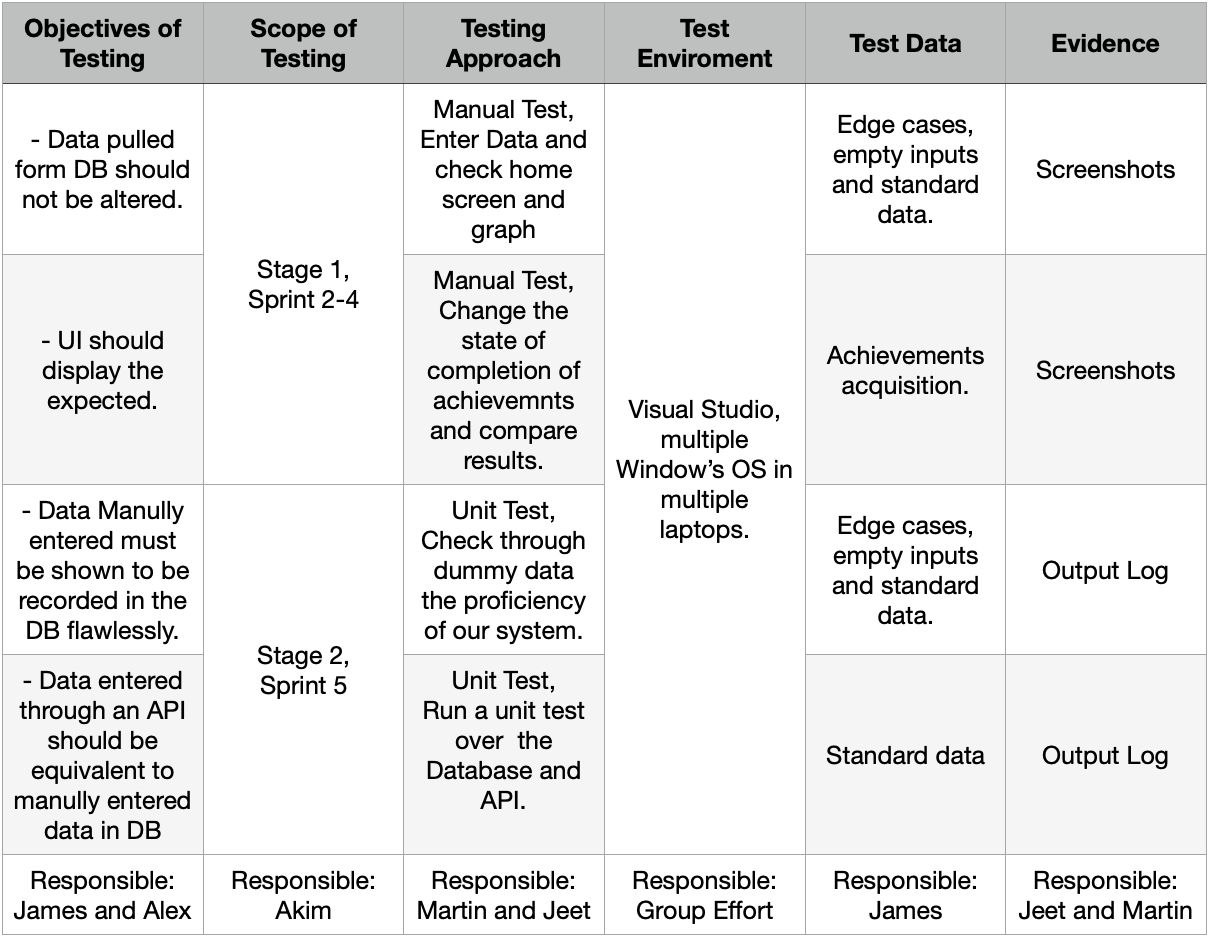
\includegraphics[width = 1\linewidth]{Test Design.jpg}
  \caption{Test Plan Design}
    \label{fig:TestDesign}
\end{figure}
\pagebreak
\subsection{Manual Testing}

\begin{figure}[!ht]
  \centering
  \begin{subfigure}{0.4\linewidth}
    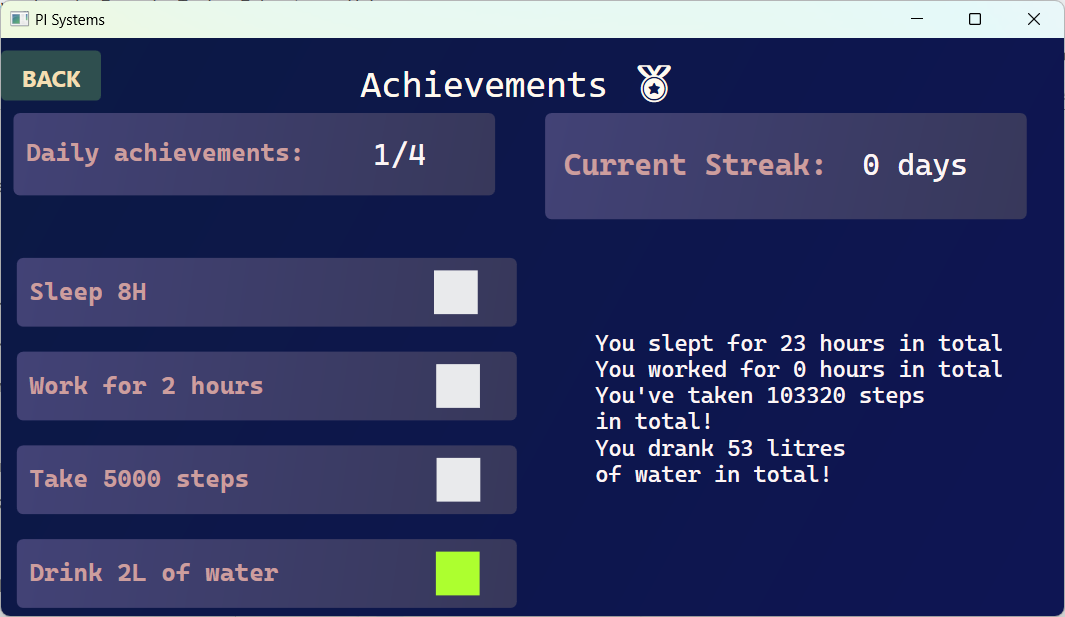
\includegraphics[width=\linewidth]{achievementCorrect.png}
    \caption{Achievement Correct}
    \label{fig:ManualTest1.1}
  \end{subfigure}
  \hfill
  \begin{subfigure}{0.4\linewidth}
    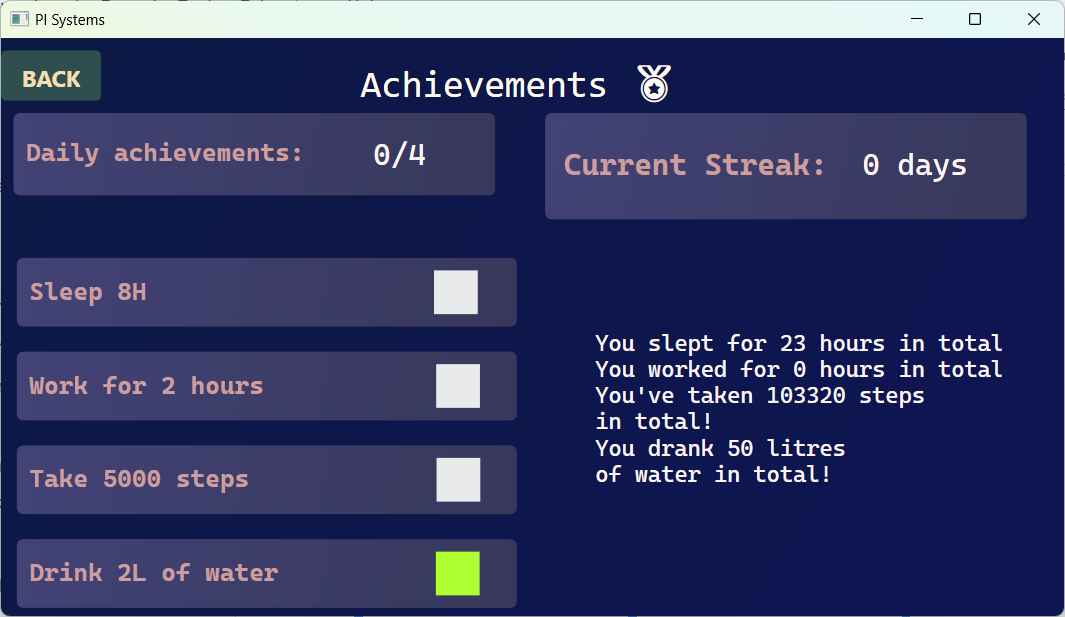
\includegraphics[width=\linewidth]{achievementIncorrect.png}
    \caption{Achievement Incorrect}
    \label{fig:ManualTest1.2}
  \end{subfigure}
  \caption{Achievement Test}
  \label{fig:ManualTest1}
\end{figure}




\begin{figure}[!ht]
\centering
    
\includegraphics[width=0.8\linewidth]{decimalPointError.png}
\caption{Decimal Point Error}
\label{fig:ManualTest2}
\end{figure}

\begin{figure}[!ht]
\centering
    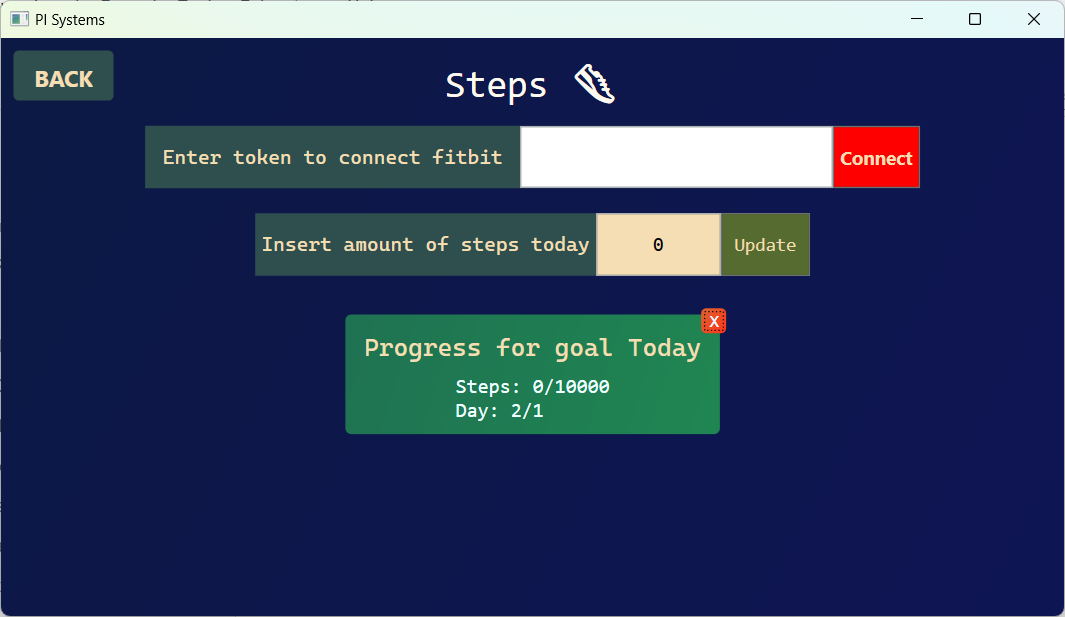
\includegraphics[width=0.6\linewidth]{goalNotExpiring.png}
\caption{Goal Not Expiring}
\label{fig:ManualTest3}
\end{figure}

\pagebreak
\subsection{Unit Testing}


\newpage
\section{Appendix: Group Contribution Form}

\begin{table}[!ht]
\centering
\begin{tabular}{|p{1.5cm}|p{1.5cm}|p{3cm}|p{6cm}|}
\hline
\textbf{Name} & \textbf{Email} & \textbf{Contribution} & \textbf{Comment} \\
\hline
\textbf{Akim} &  ak3625 & 10 & Led meetings, essentially managed the whole project and was constantly giving feedback  \\
\hline
\textbf{Alex} & ah3208 & 8 & Good group member who fully participated \\
\hline
\textbf{James} & js4209 & 8 & Good group member who fully participated\\
\hline
\textbf{Jeet} & jm3522 & 10 & Took on most of the technical element of the project and was always working on the program\\
\hline
\textbf{Katrya} & kd794 & 8 & Good group member who fully participated\\
\hline
\textbf{Martin} & md2353 & 8 & Good group member who fully participated \\
\hline
\textbf{Ollie} & ov247 & 8 & Good group member who fully participated\\
\hline
\textbf{Tom} & tb2301 & 8 & Good group member who fully participated\\
\hline
\textbf{Thang} & ctn32 & 8 & Good group member who fully participated\\
\hline
\end{tabular}
\end{table}

\newpage
\section{Appendix: Contribution Table}

\begin{table}[!ht]
\begin{adjustwidth}{-3cm}{-3cm}
\centering
\begin{tabular}{|p{1.5cm}|p{3.1cm}|p{3cm}|p{3cm}|p{3cm}|p{3cm}|}
\hline
\textbf {Name} & \textbf{Week 1} & \textbf{Week 2} & \textbf{Week 3} & \textbf{Week 4} & \textbf{Week 5} \\
\hline
\textbf{Akim} & Led meeting, took down minutes, created Github Repo, created latex report framework and created and ran a survey& Led meeting, took down minutes, assigned workload, created UI diagram and presented to the Technical Team &  Led meeting, took down minutes, assigned workload and reviewed the documentation &  Led meeting, took down minutes, assigned workload and reviewed the documentation& Led meeting, took down minutes, assigned workload and reviewed and improved the documentation \\
\hline
\textbf{Alex} & Researched PI structures, found out what data to collect and researched the effective of PI systems & Created UI diagram with Akim & Attempted to work on UI  & Documented the functional requirements and justifications for each & Adding requirements to the Design section \\
\hline
\textbf{James} & Reviewed, commented and created priorities to each given requirement and added some additional ones & Worked on Steps and Work UI and added some functionality & Added more functionality to the work page e.g. timers & Added ability to delete work goals and all work done adds to a total work value & Reviewed and provided feedback on the report \\
\hline
\textbf{Jeet} & Interviewed people about PI systems and created transcript about key data gathered & Made database ERD, UML class diagrams, researched SCRUM and finished Menu UI & Updated the way databases work and created goal table that works with the UI & Connected Fitbit API with the app, where the user can input their token to download all their data & Made a Work table that works with James' UI and added some functionality to the update button \\
\hline
\textbf{Katrya} & Made table comparing appropriate languages for the UI design & Researched databases and C\# connections & N/A & Created achievements UI and functionality & Polished up achievements UI \\
\hline
\end{tabular}
\end{adjustwidth}
\end{table}


\newpage

\begin{table}[!ht]
\begin{adjustwidth}{-3cm}{-3cm}
\centering
\begin{tabular}{|p{1.5cm}|p{3.1cm}|p{3cm}|p{3cm}|p{3cm}|p{3cm}|}
\hline
\textbf{Martin} & Made summary on research into Fitbit software & Wrote Introduction section & Wrote Agile software section of report & Started Testing section and updated Agile section & Wrote reflection, conclusion sections and updated Agile section  \\
\hline
\textbf{Ollie} & Made summary on two articles on PI systems & Created the UI, made theme and researched graphing & Applied graphs to the UI with each statistic & Connected graphs to database and added the ability to change time period & Screenshotted prototype 1, integrated work into graphs and polished graphs UI\\
\hline
\textbf{Tom} & Made summary on research into Garmin software & Created basic program showing how Fitbit API could be used & Rephrased specification section and added more detail to documentation & More rephrasing in specification section, finished non-functional requirements and polished other parts & Updated specification section to reflect our program, requirements table \\
\hline
\textbf{Thang} &  Made summary on two articles on PI systems & Wrote first half of specification section and drafted second & Started writing design section and finished ERD description & Completed design description with UML models and added non-functional requirement justifications & Adjusted UML description and finished UI design description \\
\hline
\end{tabular}
\end{adjustwidth}
\end{table}


\newpage
\section{Appendix: Minutes}
\newcommand{\tightlist}{}

\hypertarget{minutes-from-2503}{%
\subsection{Minutes From 25/03}\label{minutes-from-2503}}

\hypertarget{attendance}{%
\subsubsection{Attendance}\label{attendance}}

\begin{itemize}
\tightlist
\item
  Taking attendance.
\end{itemize}

\hypertarget{meeting-notes}{%
\subsubsection{Meeting Notes}\label{meeting-notes}}

\begin{itemize}
\tightlist
\item
  James is currently responsible for making the group contribution table
  and the attendance table.
\item
  The plan for the first sprint was discussed as a group discussion. See
  the next section for details.
\item
  With everything discussed, team members have started working on their
  tasks.
\end{itemize}

\hypertarget{first-sprint-2503-0104}{%
\subsubsection{First Sprint (25/03 ---
01/04)}\label{first-sprint-2503-0104}}

\textbf{Tasks}:

\begin{enumerate}
\def\labelenumi{\arabic{enumi}.}
\tightlist
\item
  \textbf{Gather Articles:}

  \begin{itemize}
  \tightlist
  \item
    Each member finds two articles and provides a brief summary of each.
  \item
    Everyone must research at least one article by this Wednesday.
  \item
    \textbf{Responsible:}

    \begin{itemize}
    \tightlist
    \item
      Alex --- will provide at least one article from the specification.
    \item
      Thang
    \item
      Ollie
    \end{itemize}
  \end{itemize}
\item
  \textbf{Interviewing:}

  \begin{itemize}
  \tightlist
  \item
    \textbf{Responsible:}

    \begin{itemize}
    \tightlist
    \item
      Jeet --- for live interviewing and taking transcripts.
    \item
      Akim --- creates and distributes a Google Form/survey.
    \end{itemize}
  \end{itemize}
\item
  \textbf{Market Research:}

  \begin{itemize}
  \tightlist
  \item
    Potentially provide reference(s).
  \item
    \textbf{Responsible:}

    \begin{itemize}
    \tightlist
    \item
      Tom --- researches one competitor and provides a summary of his
      findings.
    \item
      Martin --- researches another competitor and provides a summary of
      his findings.
    \end{itemize}
  \end{itemize}
  \newpage
\item
  \textbf{Draft the Initial Requirements:}

  \begin{itemize}
  \tightlist
  \item
    \textbf{Responsible:} James
  \end{itemize}
\item
  \textbf{Start the Report in LaTeX:}

  \begin{itemize}
  \tightlist
  \item
    \textbf{Responsible:} Akim --- provides the initial framework.
  \end{itemize}
\item
  \textbf{Research Programming Languages:}

  \begin{itemize}
  \tightlist
  \item
    \textbf{Responsible:} Katrya --- to research languages including
    Python, C\#, Java, C++, and JavaScript (in case we decide to create
    a website instead of implementing on PC), and others if necessary.
    Create a table listing different characteristics to compare and
    contrast, and provide a brief summary/conclusion.
  \end{itemize}
\end{enumerate}

\hypertarget{next-week-discussion-points}{%
\subsubsection{Next Week Discussion
Points}\label{next-week-discussion-points}}

\begin{itemize}
\tightlist
\item
  Finalize the initial version of the spec, including:

  \begin{itemize}
  \tightlist
  \item
    What are the requirements?
  \item
    Deciding on the PI to use.
  \end{itemize}
\item
  Which language to use? Is Python suited for the job? Consider if it's
  only suitable as a prototype.
\end{itemize}

\hypertarget{minutes-from-0104}{%
\subsection{Minutes From 01/04}\label{minutes-from-0104}}

\hypertarget{attendance-1}{%
\subsubsection{Attendance}\label{attendance-1}}

\begin{itemize}
\tightlist
\item
  Taking attendance.
\end{itemize}

\hypertarget{discussion-topics}{%
\subsubsection{Discussion Topics}\label{discussion-topics}}

\begin{itemize}
\tightlist
\item
  \textbf{Requirements Table:} Discussion on the requirements table
  prepared by James.
\item
  \textbf{SCRUM Master:} Jeet has volunteered to be the SCRUM master,
  with responsibilities including in-depth SCRUM research and advising
  on future strategy steps.
\item
  \textbf{Meeting Leader:} Akim has volunteered to be the meeting leader
  for all future meetings.
\item
  \textbf{Writing Assignments:}

  \begin{itemize}
  \tightlist
  \item
    Alex will complete an article from the specification by today.
  \item
    Alex, Ollie, and Thang are tasked with inserting references into the
    requirements table by the end of the week.
  \end{itemize}
\item
  \textbf{Programming Language:} C\# has been selected as the
  programming language for the project.
\item
  \textbf{Development Roles:}

  \begin{itemize}
  \tightlist
  \item
    Jeet and Ollie have been appointed as front-end developers.
  \end{itemize}
\item
  \textbf{Sprint Planning:} Discussion about the second sprint.
\end{itemize}

\hypertarget{second-sprint-0104-0804}{%
\subsubsection{Second Sprint (01/04 ---
08/04)}\label{second-sprint-0104-0804}}

\textbf{Tasks}:

\begin{enumerate}
\def\labelenumi{\arabic{enumi}.}
\tightlist
\item
  \textbf{Create a UI Diagram by Wednesday:}

  \begin{itemize}
  \tightlist
  \item
    \textbf{Responsible:}

    \begin{itemize}
    \tightlist
    \item
      Akim
    \item
      Alex
    \end{itemize}
  \end{itemize}
\item
  \textbf{Create Framework for the Project on GitHub:}

  \begin{itemize}
  \tightlist
  \item
    \textbf{Responsible:}

    \begin{itemize}
    \tightlist
    \item
      Jeet
    \end{itemize}
  \end{itemize}
\item
  \textbf{After the UI Diagram is Finished, Create a Coding Plan:}

  \begin{itemize}
  \tightlist
  \item
    It should include both front-end and back-end.
  \item
    \textbf{Responsible:}

    \begin{itemize}
    \tightlist
    \item
      Jeet
    \item
      Ollie
    \item
      James
    \end{itemize}
  \end{itemize}
\item
  \textbf{Potentially Start the UI for the Menu:}

  \begin{itemize}
  \tightlist
  \item
    \textbf{Responsible:}

    \begin{itemize}
    \tightlist
    \item
      Jeet and/or Ollie
    \end{itemize}
  \end{itemize}
\item
  \textbf{Research APIs:}

  \begin{itemize}
  \tightlist
  \item
    Create a small program with comments showing off basic
    functionality.
  \item
    Share the program on GitHub in the \texttt{research} directory
    (create if doesn't exist).
  \item
    \textbf{Responsible:}

    \begin{itemize}
    \tightlist
    \item
      Tom
    \end{itemize}
  \end{itemize}
\item
  \textbf{Start Writing the Content of the Report:}

  \begin{itemize}
  \tightlist
  \item
    \textbf{The Introduction section:}

    \begin{itemize}
    \tightlist
    \item
      Martin
    \end{itemize}
  \item
    \textbf{The Software Requirements Specification:}

    \begin{itemize}
    \tightlist
    \item
      Thang
    \end{itemize}
  \end{itemize}
\item
  \textbf{Create a Basic DB Using SQL and C\#:}

  \begin{itemize}
  \tightlist
  \item
    A small program with comments that describes basic operations.
  \item
    Share the program on GitHub in the \texttt{research} directory
    (create if doesn't exist).
  \item
    \textbf{Responsible:}

    \begin{itemize}
    \tightlist
    \item
      Katrya
    \end{itemize}
  \end{itemize}
\end{enumerate}

\hypertarget{minutes-from-0804}{%
\subsection{Minutes From 08/04}\label{minutes-from-0804}}

\hypertarget{attendance-2}{%
\subsubsection{Attendance}\label{attendance-2}}

\begin{itemize}
\tightlist
\item
  Taking attendance.
\end{itemize}

\hypertarget{discussion-topics-1}{%
\subsubsection{Discussion Topics}\label{discussion-topics-1}}

\begin{itemize}
\tightlist
\item
  \textbf{Discussing the Report:}

  \begin{itemize}
  \tightlist
  \item
    Martin has completed his task and will merge the report branch into
    the master after the meeting.
  \item
    Thang has completed his task and will upload his work on GitHub by
    the end of today.
  \end{itemize}
\item
  \textbf{Presentations:}

  \begin{itemize}
  \tightlist
  \item
    Jeet presented the UML diagram.
  \item
    Jeet presented the ERD.
  \item
    Jeet walked everyone through the code.
  \item
    Oliver presented how the graphs will be implemented.
  \end{itemize}
\item
  \textbf{APIs:}

  \begin{itemize}
  \tightlist
  \item
    Tom discussed the research he has done on APIs and will upload it to
    GitHub today.
  \end{itemize}
\end{itemize}

\hypertarget{third-sprint-0804-1504}{%
\subsubsection{Third Sprint (08/04 ---
15/04)}\label{third-sprint-0804-1504}}

\textbf{Coding tasks}:

\begin{enumerate}
\def\labelenumi{\arabic{enumi}.}
\tightlist
\item
  Potentially fully code the \textbf{Graphs} part.

  \begin{itemize}
  \tightlist
  \item
    \textbf{Responsible:}

    \begin{itemize}
    \tightlist
    \item
      Oliver
    \end{itemize}
  \end{itemize}
\item
  Potentially fully code the \textbf{Achievements} part.

  \begin{itemize}
  \tightlist
  \item
    \textbf{Responsible:}

    \begin{itemize}
    \tightlist
    \item
      Alex
    \end{itemize}
  \end{itemize}
\item
  Potentially fully code the \textbf{Work} part:

  \begin{itemize}
  \tightlist
  \item
    \textbf{Responsible:}

    \begin{itemize}
    \tightlist
    \item
      James
    \end{itemize}
  \end{itemize}
\item
  Fully implement the \textbf{goals for all metrics} apart from Work.

  \begin{itemize}
  \tightlist
  \item
    \textbf{Responsible:}

    \begin{itemize}
    \tightlist
    \item
      Jeet
    \end{itemize}
  \end{itemize}
\item
  Implement the \textbf{API for Steps}:

  \begin{itemize}
  \tightlist
  \item
    \textbf{Responsible:}

    \begin{itemize}
    \tightlist
    \item
      Akim or Jeet (to be decided)
    \end{itemize}
  \end{itemize}
\item
  Consider \textbf{changing the DB design}:

  \begin{itemize}
  \tightlist
  \item
    \textbf{Responsible:}

    \begin{itemize}
    \tightlist
    \item
      Jeet
    \end{itemize}
  \end{itemize}
\end{enumerate}

\textbf{Report tasks:}

\begin{enumerate}
\def\labelenumi{\arabic{enumi}.}
\setcounter{enumi}{6}
\tightlist
\item
  \textbf{Go through the report and give feedback} to Thang and Martin:

  \begin{itemize}
  \tightlist
  \item
    \textbf{Responsible:}

    \begin{itemize}
    \tightlist
    \item
      Akim
    \end{itemize}
  \end{itemize}
  \newpage
\item
  Go through the report part of the spec and \textbf{allocate work} to
  Tom:

  \begin{itemize}
  \tightlist
  \item
    \textbf{Deadline:} Wednesday
  \item
    \textbf{Responsible:}

    \begin{itemize}
    \tightlist
    \item
      Akim
    \end{itemize}
  \end{itemize}
\item
  Complete the \textbf{Introduction Section}:

  \begin{itemize}
  \tightlist
  \item
    \textbf{Responsible:}

    \begin{itemize}
    \tightlist
    \item
      Martin
    \end{itemize}
  \end{itemize}
\item
  Start the \textbf{SCRUM Section}:

  \begin{itemize}
  \tightlist
  \item
    \textbf{Responsible:}

    \begin{itemize}
    \tightlist
    \item
      Martin
    \end{itemize}
  \end{itemize}
\item
  Start the \textbf{Design Section}:

  \begin{itemize}
  \tightlist
  \item
    \textbf{Responsible:}

    \begin{itemize}
    \tightlist
    \item
      Thang
    \end{itemize}
  \end{itemize}
\end{enumerate}

\hypertarget{minutes-from-1504}{%
\subsection{Minutes From 15/04}\label{minutes-from-1504}}

\hypertarget{attendance-3}{%
\subsubsection{Attendance}\label{attendance-3}}

\begin{itemize}
\tightlist
\item
  Taking attendance.
\end{itemize}

\hypertarget{discussion-topics-2}{%
\subsubsection{Discussion Topics}\label{discussion-topics-2}}

\begin{itemize}
\tightlist
\item
  \textbf{Ollie's Presentation on Graphs:}

  \begin{itemize}
  \tightlist
  \item
    Ollie completed the basic version of the graphs, which currently
    lacks functionality.
  \end{itemize}
\item
  \textbf{James' Update on Database Integration:}

  \begin{itemize}
  \tightlist
  \item
    James added database integration to the Work page.
  \end{itemize}
\item
  \textbf{Jeet's Contributions:}

  \begin{itemize}
  \tightlist
  \item
    Implemented goals for all metrics.
  \item
    Simplified the database design.
  \item
    Began integrating the API.
  \end{itemize}
  \newpage
\item
  \textbf{General Discussions:}

  \begin{itemize}
  \tightlist
  \item
    The team discussed the report.
  \item
    The Scrum development process was reviewed.
  \item
    Testing plans were outlined; testing will commence after product
    completion next week.
  \item
    Reviewed the project requirements.
  \end{itemize}
\end{itemize}

\hypertarget{fourth-sprint-1504-2204}{%
\subsubsection{Fourth Sprint (15/04 ---
22/04)}\label{fourth-sprint-1504-2204}}

\textbf{Coding tasks}:

\begin{enumerate}
\def\labelenumi{\arabic{enumi}.}
\tightlist
\item
  Finish the \textbf{Graphs}.

  \begin{itemize}
  \tightlist
  \item
    \textbf{Responsible:} Ollie
  \end{itemize}
\item
  Develop the \textbf{Achievements UI} and Start \textbf{Functional
  Implementation}.

  \begin{itemize}
  \tightlist
  \item
    \textbf{Responsible:}

    \begin{itemize}
    \tightlist
    \item
      Katrya
    \item
      Potentially Jeet (see \#5)
    \end{itemize}
  \end{itemize}
\item
  Complete the \textbf{Work Section}.

  \begin{itemize}
  \tightlist
  \item
    \textbf{Responsible:}

    \begin{itemize}
    \tightlist
    \item
      Potentially James (confirmation by end of today)
    \end{itemize}
  \end{itemize}
\item
  Finish the \textbf{API Integration}.

  \begin{itemize}
  \tightlist
  \item
    \textbf{Responsible:}

    \begin{itemize}
    \tightlist
    \item
      Jeet
    \end{itemize}
  \end{itemize}
\item
  Assist with \textbf{Achievements Functionality}.

  \begin{itemize}
  \tightlist
  \item
    \textbf{Responsible:}

    \begin{itemize}
    \tightlist
    \item
      Jeet
    \end{itemize}
  \end{itemize}
\end{enumerate}

\textbf{Report tasks}:

\begin{enumerate}
\def\labelenumi{\arabic{enumi}.}
\setcounter{enumi}{5}
\tightlist
\item
  \textbf{Review} the Report and \textbf{Provide Feedback}.

  \begin{itemize}
  \tightlist
  \item
    \textbf{Responsible:}

    \begin{itemize}
    \tightlist
    \item
      Akim
    \end{itemize}
  \end{itemize}
\newpage
\item
  \textbf{Assign Tasks} for Martin and Alex.

  \begin{itemize}
  \tightlist
  \item
    \textbf{Deadline:}

    \begin{itemize}
    \tightlist
    \item
      Wednesday
    \end{itemize}
  \item
    \textbf{Responsible:}

    \begin{itemize}
    \tightlist
    \item
      Akim
    \end{itemize}
  \end{itemize}
\item
  Finish the \textbf{Requirements Section}.

  \begin{itemize}
  \tightlist
  \item
    \textbf{Responsible:}

    \begin{itemize}
    \tightlist
    \item
      Tom
    \end{itemize}
  \end{itemize}
\item
  Finish the \textbf{Design Section}.

  \begin{itemize}
  \tightlist
  \item
    \textbf{Responsible:}

    \begin{itemize}
    \tightlist
    \item
      Thang
    \end{itemize}
  \end{itemize}
\item
  \textbf{Update the Scrum Section}.

  \begin{itemize}
  \tightlist
  \item
    \textbf{Responsible:}

    \begin{itemize}
    \tightlist
    \item
      Martin
    \end{itemize}
  \end{itemize}
\end{enumerate}

\hypertarget{minutes-from-1904}{%
\subsection{Minutes From 19/04}\label{minutes-from-1904}}

\hypertarget{attendance-4}{%
\subsubsection{Attendance}\label{attendance-4}}

\begin{itemize}
\tightlist
\item
  Taking attendance.
\end{itemize}

\hypertarget{discussion-topics-3}{%
\subsubsection{Discussion Topics}\label{discussion-topics-3}}

\begin{itemize}
\tightlist
\item
  Discussing progress.
\item
  \textbf{API}:

  \begin{itemize}
  \tightlist
  \item
    Jeet is almost done, will finish the API integration by Sunday.
  \end{itemize}
\item
  Start the software testing section of the report.

  \begin{itemize}
  \tightlist
  \item
    \textbf{Responsible}:

    \begin{itemize}
    \tightlist
    \item
      Martin
    \end{itemize}
  \end{itemize}
\item
  Everyone else is continuing with their work for Monday.
\end{itemize}

\hypertarget{minutes-from-2204}{%
\subsection{Minutes From 22/04}\label{minutes-from-2204}}

\hypertarget{attendance-5}{%
\subsubsection{Attendance}\label{attendance-5}}

\begin{itemize}
\tightlist
\item
  Taking attendance.
\end{itemize}

\hypertarget{progress-review-and-final-sprint-2204-0305}{%
\subsubsection{Progress Review and Final Sprint (22/04 ---
03/05)}\label{progress-review-and-final-sprint-2204-0305}}

\textbf{Coding}:

\begin{itemize}
\item
  Ollie has finished the \textbf{Graphs} except for the Work part, which
  has not been fully implemented yet by James.
\item
  \textbf{Achievements UI} has been completed, but \textbf{not the
  functional part}, which will be done by Wednesday.

  \begin{itemize}
  \tightlist
  \item
    \textbf{Responsible}: Katrya
  \item
    \textbf{Deadline}: Wednesday
  \end{itemize}
\item
  The \textbf{Work} part is not fully finished yet, it has to be linked
  to the DB and properly merged with the rest of the code by Wednesday.

  \begin{itemize}
  \tightlist
  \item
    \textbf{Responsible}: James
  \item
    \textbf{Backup}: Ollie
  \item
    \textbf{Deadline}: Wednesday
  \end{itemize}
\item
  Jeet has \textbf{fully integrated the API part}.

  \begin{itemize}
  \tightlist
  \item
    Some \textbf{bugs} have been discovered by the product owner; they
    \textbf{will be fixed shortly}.
  \end{itemize}
\item
  Jeet will \textbf{merge everything into the master branch} by
  Wednesday.

  \begin{itemize}
  \tightlist
  \item
    \textbf{Responsible}: Jeet
  \item
    \textbf{Deadline}: Wednesday
  \end{itemize}
\item
  Jeet will implement the table in the DB for Achievements by Friday.

  \begin{itemize}
  \tightlist
  \item
    \textbf{Responsible}: Jeet
  \item
    \textbf{Deadline}: Friday
  \end{itemize}
\end{itemize}

\newpage
\textbf{Report}:

\begin{itemize}
\tightlist
\item
  Tom has almost finished the \textbf{Requirements section}, however it
  has to be redone in the form of a table.

  \begin{itemize}
  \tightlist
  \item
    \textbf{Responsible}: Tom
  \item
    \textbf{Deadline}: Wednesday
  \end{itemize}
\item
  Thang and Alex have not been able to complete the \textbf{Design
  section} by today, but they will fully complete it and push to GitHub
  by no later than Wednesday.

  \begin{itemize}
  \tightlist
  \item
    \textbf{Responsible}: Thang, Alex
  \item
    \textbf{Deadline}: Wednesday
  \end{itemize}
\item
  Martin has updated the \textbf{Scrum section} for the previous week,
  and will do the same for this week.

  \begin{itemize}
  \tightlist
  \item
    \textbf{Responsible}: Martin
  \end{itemize}
\item
  Start the \textbf{Reflection and Conclusion} section of the report

  \begin{itemize}
  \tightlist
  \item
    \textbf{Responsible}: Martin
  \end{itemize}
\item
  Give feedback on the \textbf{Testing section} and let Martin know what
  to do next

  \begin{itemize}
  \tightlist
  \item
    \textbf{Responsible}: Akim
  \item
    \textbf{Deadline}: Wednesday
  \end{itemize}
\end{itemize}

\hypertarget{minutes-from-2904}{%
\subsection{Minutes From 29/04}\label{minutes-from-2904}}

\hypertarget{attendance-6}{%
\subsubsection{Attendance}\label{attendance-6}}

\begin{itemize}
\tightlist
\item
  Taking attendance.
\end{itemize}

\hypertarget{progress-review-and-report-finalization}{%
\subsubsection{Progress Review and Report
Finalization}\label{progress-review-and-report-finalization}}

\begin{itemize}
\tightlist
\item
  Upload the \textbf{updated ERD} to the Google doc.

  \begin{itemize}
  \tightlist
  \item
    \textbf{Responsible}: Jeet
  \end{itemize}
\item
  Update the \textbf{ERD} in the report.

  \begin{itemize}
  \tightlist
  \item
    \textbf{Responsible}: Thang
  \end{itemize}
\item
  Insert \textbf{ARQ/SRQ notation} to the rest of Thang's Design
  section.

  \begin{itemize}
  \tightlist
  \item
    \textbf{Responsible}: Alex
  \end{itemize}
\item
  Complete the \textbf{Requirements} section now.

  \begin{itemize}
  \tightlist
  \item
    \textbf{Responsible}: Tom
  \end{itemize}
\item
  Update \textbf{SCRUM} and complete the \textbf{Testing} section.

  \begin{itemize}
  \tightlist
  \item
    \textbf{Responsible}: Martin
  \end{itemize}
\item
  Go through the report and give feedback.

  \begin{itemize}
  \tightlist
  \item
    \textbf{Responsible}: James, Akim
  \end{itemize}
\item
  Include \textbf{appendices} in the report.

  \begin{itemize}
  \tightlist
  \item
    \textbf{Responsible}: Akim
  \end{itemize}
\item
  Ollie successfully integrated the \textbf{work section with the
  graphs} and implemented \textbf{dynamic upper bound} for the graphs.
\end{itemize}

\end{document}

